
\begin{table*}[t]\small
\renewcommand\tabcolsep{2pt}
\centering
\caption{Final Accuracy Rate (↑). The best scores for our methods are in boldface, and the best scores for baselines are underlined.}
\vspace{-2ex}
\label{tableaccuracy}
\begin{tabular}{l|ccc|ccc|ccc|ccc}
\hline
Datasets & \multicolumn{3}{c|}{Split CIFAR10 (\%)} & \multicolumn{3}{c|}{Split CIFAR100 (\%)}& \multicolumn{3}{c|}{Split MiniImageNet (\%)} & \multicolumn{3}{c}{Split TinyImageNet (\%)}\\ \hline
Buffer & \multicolumn{1}{c|}{100} & \multicolumn{1}{c|}{200} & \multicolumn{1}{c|}{500} & \multicolumn{1}{c|}{1000}    & \multicolumn{1}{c|}{2000} & \multicolumn{1}{c|}{5000} & \multicolumn{1}{c|}{1000} & \multicolumn{1}{c|}{2000}     &\multicolumn{1}{c|}{5000} & \multicolumn{1}{c|}{2000} & \multicolumn{1}{c|}{4000} & 10000     \\ \hline
IID          & \multicolumn{3}{c|}{58.1\scriptsize±2.5}                                  & \multicolumn{3}{c|}{17.3\scriptsize±0.8}                                     & \multicolumn{3}{c|}{18.2\scriptsize±1.1} & \multicolumn{3}{c}{17.3\scriptsize±1.7}                                    \\
IID++~\cite{caccia2021new}          & \multicolumn{3}{c|}{64.2\scriptsize±2.1}                                  & \multicolumn{3}{c|}{23.5\scriptsize±0.8}                                     & \multicolumn{3}{c|}{20.7\scriptsize±1.0} & \multicolumn{3}{c}{19.1\scriptsize±1.3}                                    \\
FINE-TUNE          & \multicolumn{3}{c|}{17.9\scriptsize±0.4}                                  & \multicolumn{3}{c|}{5.9\scriptsize±0.2}                                     & \multicolumn{3}{c|}{4.3\scriptsize±0.2} & \multicolumn{3}{c}{4.3\scriptsize±0.2}                                    \\\hline

ER~\cite{rolnick2019experience} (NeurIPS2019) & 33.8\scriptsize±3.2& 41.7\scriptsize±2.8                 & 46.0\scriptsize±3.5                 & 17.6\scriptsize±0.9                  & 19.7\scriptsize±1.6                  & 20.9\scriptsize±1.2 & 13.4\scriptsize±0.9                   & 16.5\scriptsize±0.9                  & 16.2\scriptsize±1.7 & 6.1\scriptsize±0.5                   & 8.5\scriptsize±0.7                  & 8.9\scriptsize±0.6\\
GSS~\cite{aljundi2019gradient} (NeurIPS2019) & 23.1\scriptsize±3.9& 28.3\scriptsize±4.6                 & 36.3\scriptsize±4.1                 & 16.9\scriptsize±1.4                  & 19.0\scriptsize±1.8                  & 20.1\scriptsize±1.1 & 13.9\scriptsize±1.0                   & 14.6\scriptsize±1.1                  & 15.5\scriptsize±0.9 & /                   & /                  & /\\
GMED~\cite{jin2021gradient} (NeurIPS2021) & 32.8\scriptsize±4.7& 43.6\scriptsize±5.1                 & 52.5\scriptsize±3.9                 & 18.8\scriptsize±0.7                  & 21.1\scriptsize±1.2                  & 23.0\scriptsize±1.5 & 15.3\scriptsize±1.3                   & 18.0\scriptsize±0.8                  & 19.6\scriptsize±1.0 & 7.0\scriptsize±0.9                   & 10.2\scriptsize±0.7                  & 11.3\scriptsize±1.2\\
MIR~\cite{aljundi2019online} (NeurIPS2019)& 34.8\scriptsize±3.3& 40.3\scriptsize±3.3                 & 42.6\scriptsize±1.7                 & 18.1\scriptsize±0.7                  & 20.3\scriptsize±1.6                  & 21.6\scriptsize±1.7 & 14.8\scriptsize±1.1                   & 17.2\scriptsize±0.8                  & 17.2\scriptsize±1.2 & 4.9\scriptsize±0.6                   & 6.3\scriptsize±0.6                  & 6.4\scriptsize±0.7\\
ASER~\cite{shim2021online} (AAAI2021) & 33.7\scriptsize±3.7& 31.6\scriptsize±3.4                 & 42.1\scriptsize±3.0                 & 16.1\scriptsize±1.1                  & 17.7\scriptsize±0.7                  & 18.9\scriptsize±1.0 & 13.8\scriptsize±0.9                   & 16.1\scriptsize±0.9                  & 18.1\scriptsize±1.1 & 5.3\scriptsize±0.3                   & 9.6\scriptsize±0.8                  & 8.1\scriptsize±0.8\\
A-GEM~\cite{chaudhry2018efficient} (ICLR2019)& 17.5\scriptsize±1.7& 17.4\scriptsize±2.1                 & 17.9\scriptsize±0.7                 & 5.6\scriptsize±0.5                  & 5.4\scriptsize±0.7                  & 4.6\scriptsize±1.0 & 4.7\scriptsize±1.1                   & 5.0\scriptsize±2.3                  & 4.8\scriptsize±0.8 & /                   & /                  & /\\
ER-WA~\cite{zhao2020maintaining} (CVPR2020)& 36.9\scriptsize±2.9& 42.5\scriptsize±3.4                 & 48.6\scriptsize±2.7                 & 21.7\scriptsize±1.2                  & 23.6\scriptsize±0.9                  & 24.0\scriptsize±1.8 & 17.1\scriptsize±0.9                   & 18.9\scriptsize±1.4                  & 18.5\scriptsize±1.5 & 9.2\scriptsize±0.7                   & 11.6\scriptsize±1.3                  & 11.4\scriptsize±1.6\\
DER++~\cite{buzzega2020dark} (NeurIPS2020)& 40.9\scriptsize±1.4& 45.3\scriptsize±1.7                 & 52.8\scriptsize±2.2                 & 17.2\scriptsize±1.1                  & 19.5\scriptsize±1.2                  & 20.2\scriptsize±1.3 & 14.8\scriptsize±0.7                   & 16.1\scriptsize±1.3                  & 15.5\scriptsize±1.3 & 6.8\scriptsize±0.4                   & 8.7\scriptsize±0.7                  & 9.2\scriptsize±0.7\\
SS-IL~\cite{ahn2021ss} (ICCV2021) & 36.8\scriptsize±2.1 & 42.2\scriptsize±1.4                 &  44.8\scriptsize±1.6                 & 21.9\scriptsize±1.1                  & 24.5\scriptsize±1.4                  & 24.7\scriptsize±1.0 & 19.7\scriptsize±0.9                   & 21.7\scriptsize±1.0                  & 24.4\scriptsize±1.6 &\underline{13.2\scriptsize±0.8}                   & \underline{15.2\scriptsize±1.0}                  & \underline{18.7\scriptsize±0.7}\\
SCR~\cite{mai2021supervised} (CVPR-W2021) & 35.0\scriptsize±2.9& 45.4\scriptsize±1.0                 & 55.7\scriptsize±1.6                 & 16.2\scriptsize±1.3                  & 18.2\scriptsize±0.8                  & 19.3\scriptsize±1.0 & 14.7\scriptsize±1.9                   & 16.8\scriptsize±0.6                  & 18.6\scriptsize±0.5 & 9.9\scriptsize±0.4                   & 12.6\scriptsize±0.6                  & 11.1\scriptsize±0.5\\
ER-DVC~\cite{gu2022not} (CVPR2022) & 36.3\scriptsize±2.6 & 45.4\scriptsize±1.4                 &  50.6\scriptsize±2.9                & 19.7\scriptsize±0.7                  & 22.1\scriptsize±0.9                  & 24.1\scriptsize±0.8 & 15.4\scriptsize±0.7                   & 17.2\scriptsize±0.8                  & 19.1\scriptsize±0.9 & 7.6\scriptsize±0.5                   & 9.9\scriptsize±0.7                  & 10.4\scriptsize±0.7\\
OCM~\cite{guo2022online} (ICML2022) & {44.4\scriptsize±1.5} & {49.9\scriptsize±1.8}                 &  {55.8\scriptsize±2.3}                & 20.6\scriptsize±1.2                  & 22.1\scriptsize±1.0                  & 22.7\scriptsize±1.4 & 13.6\scriptsize±0.7                   & 16.5\scriptsize±0.5                  & 19.2\scriptsize±0.7 & 8.6\scriptsize±0.8                   & 11.9\scriptsize±0.9                  & 12.1\scriptsize±0.6\\
ER-ACE~\cite{caccia2021new} (ICLR2022)   & 44.3\scriptsize±1.5 & 49.7\scriptsize±2.4                & 54.9\scriptsize±1.4                 & {23.1\scriptsize±0.8}                &{24.8\scriptsize±0.9}                  & {27.0\scriptsize±1.2} & {20.3\scriptsize±1.3}                   & {24.8\scriptsize±1.1}                  & {26.2\scriptsize±1.0} & 9.5\scriptsize±0.5                   & 13.7\scriptsize±0.7                  & 18.2\scriptsize±0.5\\
OBC~\cite{chrysakisonline} (ICLR2023)   & 40.5\scriptsize±2.1  & 46.4\scriptsize±1.6  & 53.4\scriptsize±2.3                 & 22.1\scriptsize±0.6  & 24.0\scriptsize±1.3  & 26.3\scriptsize±1.0 & 16.4\scriptsize±1.4  & 19.5\scriptsize±1.5  & 21.6\scriptsize±1.4 & 9.6\scriptsize±0.5                   & 11.4\scriptsize±0.9                  & 14.6\scriptsize±1.1\\
OnPro~\cite{wei2023online} (ICCV2023)   & \underline{46.0\scriptsize±1.6}  & \underline{52.9\scriptsize±2.0}  & \underline{59.5\scriptsize±0.7}                 & 17.4\scriptsize±0.8  & 19.4\scriptsize±0.4  & 21.6\scriptsize±0.6 & 13.7\scriptsize±0.9  & 16.8\scriptsize±0.7  & 18.1\scriptsize±1.1 & 10.2\scriptsize±0.8                   & 13.6\scriptsize±0.7                  & 16.5\scriptsize±0.4\\
UER~\cite{lin2023uer} (ACMMM2023)   & {41.5\scriptsize±1.4}& {49.2\scriptsize±1.7}                & {55.8\scriptsize±1.9}                 & \underline{24.6\scriptsize±0.8}                &\underline{27.0\scriptsize±0.5}                  & \underline{29.6\scriptsize±1.1} & \underline{21.9\scriptsize±1.3}                   & \underline{25.1\scriptsize±1.1}                  & \underline{27.5\scriptsize±1.1} & 10.6\scriptsize±0.5                   & 13.8\scriptsize±0.7                  & 17.2\scriptsize±0.6\\
\hline
% FPCR (Equation (\ref{eq:fpcr}))   & 41.9\scriptsize±2.0& 48.3\scriptsize±2.4                & 55.8\scriptsize±1.2                 & 24.1\scriptsize±0.5           & 25.9\scriptsize±0.5          & 27.3\scriptsize±0.7 & 21.8\scriptsize±0.8                   & 24.5\scriptsize±0.9                  & 26.3\scriptsize±1.0 & {11.1\scriptsize±1.2}                   & {13.6\scriptsize±0.7}                  & {15.3\scriptsize±1.2}\\
HPCR (Algorithm \ref{alg:hpcr})   & \textbf{48.3\scriptsize±1.5}& \textbf{53.4\scriptsize±1.4}                & \textbf{60.1\scriptsize±1.1}                 & \textbf{29.1\scriptsize±0.7}                &\textbf{30.7\scriptsize±0.5}                 & \textbf{33.7\scriptsize±0.6} & \textbf{27.1\scriptsize±0.6}                   & \textbf{29.9\scriptsize±0.7}                  & \textbf{31.3\scriptsize±0.7} & \textbf{16.4\scriptsize±0.3}                   & \textbf{19.5\scriptsize±0.8}                  & \textbf{22.1\scriptsize±0.5}\\
$\hookrightarrow$PCR    & 45.4\scriptsize±1.3& 50.3\scriptsize±1.5                & 56.0\scriptsize±1.2                 & 25.6\scriptsize±0.6                &27.4\scriptsize±0.6                 & 29.3\scriptsize±1.1 & 24.2\scriptsize±0.9                   & 27.2\scriptsize±1.2                  & 28.4\scriptsize±0.9 & 12.2\scriptsize±0.9                   & 17.4\scriptsize±0.7                  & 19.6\scriptsize±0.8\\
% PCR+ (Ours)   & \textbf{47.8\scriptsize±1.5}& \textbf{51.3\scriptsize±1.6}                & \textbf{57.7\scriptsize±1.1}                 & \textbf{27.2\scriptsize±0.5}                &\textbf{29.3\scriptsize±0.7}                 & \textbf{31.6\scriptsize±0.9} & \textbf{25.6\scriptsize±1.0}                   & \textbf{28.5\scriptsize±0.5}                  & \textbf{29.8\scriptsize±0.7} & \textbf{14.8\scriptsize±0.6}                   & \textbf{18.8\scriptsize±0.5}                  & \textbf{20.8\scriptsize±0.5}\\
\hline
\end{tabular}
\vspace{-2ex}
\end{table*}


\begin{table*}[t]\small
\renewcommand\tabcolsep{1pt}
\centering
\caption{Final Accuracy Rate (↑) on Split CIFAR100 under the experimental setting of ~\cite{guo2022online}.}
\vspace{-2ex}
\label{moreaccuracy}
\begin{tabular}{l|ccc|ccc|ccc|ccc|ccc}
\hline
Methods & \multicolumn{3}{c|}{SCR~\cite{guo2022online} (\%)} & \multicolumn{3}{c|}{OCM~\cite{guo2022online} (\%)}& \multicolumn{3}{c|}{OnPro~\cite{wei2023online} (\%)} & \multicolumn{3}{c|}{PCR (\%)} & \multicolumn{3}{c}{HPCR (\%)}\\ \hline
Buffer & \multicolumn{1}{c|}{1000} & \multicolumn{1}{c|}{2000} & \multicolumn{1}{c|}{5000} & \multicolumn{1}{c|}{1000}    & \multicolumn{1}{c|}{2000} & \multicolumn{1}{c|}{5000} & \multicolumn{1}{c|}{1000} & \multicolumn{1}{c|}{2000}     &\multicolumn{1}{c|}{5000} & \multicolumn{1}{c|}{1000} & \multicolumn{1}{c|}{2000} &\multicolumn{1}{c|}{5000} & \multicolumn{1}{c|}{1000} & \multicolumn{1}{c|}{2000} & 5000     \\ \hline
$A_T$   & 26.5\scriptsize±0.2& 31.6\scriptsize±0.5                 & 36.5\scriptsize±0.2                 & 28.1\scriptsize±0.3                  & 35.0\scriptsize±0.4                  & 42.4\scriptsize±0.5 & 30.0\scriptsize±0.4                   & 35.9\scriptsize±0.6                  & 42.7\scriptsize±0.9 & 29.3\scriptsize±0.6                   & 36.3\scriptsize±0.9                  & 46.5\scriptsize±0.8 & \textbf{33.6\scriptsize±0.6}                   & \textbf{40.5\scriptsize±1.5}                  & \textbf{49.1\scriptsize±1.2} \\
\hline
\end{tabular}
\vspace{-2ex}
\end{table*}



\begin{table*}[t]\small
\renewcommand\tabcolsep{2pt}
\centering
\caption{Averaged Anytime Accuracy (↑). The best scores for our methods are in boldface, and the best for baselines are underlined.}
\vspace{-2ex}
\label{tableaaa}
\begin{tabular}{l|ccc|ccc|ccc|ccc}
\hline
Datasets & \multicolumn{3}{c|}{Split CIFAR10 (\%)} & \multicolumn{3}{c|}{Split CIFAR100 (\%)}& \multicolumn{3}{c|}{Split MiniImageNet (\%)} & \multicolumn{3}{c}{Split TinyImageNet (\%)}\\ \hline
Buffer & \multicolumn{1}{c|}{100} & \multicolumn{1}{c|}{200} & \multicolumn{1}{c|}{500} & \multicolumn{1}{c|}{1000}    & \multicolumn{1}{c|}{2000} & \multicolumn{1}{c|}{5000} & \multicolumn{1}{c|}{1000} & \multicolumn{1}{c|}{2000}     &\multicolumn{1}{c|}{5000} & \multicolumn{1}{c|}{2000} & \multicolumn{1}{c|}{4000} & 10000     \\ \hline
ER~\cite{rolnick2019experience} (NeurIPS2019) & 52.7\scriptsize±2.7& 52.1\scriptsize±3.1                 & 57.0\scriptsize±2.7                 & 25.5\scriptsize±1.1                  & 26.3\scriptsize±1.4                  & 25.3\scriptsize±1.3 & 20.1\scriptsize±0.9                   & 22.2\scriptsize±1.2                  & 19.0\scriptsize±1.5 & 11.9\scriptsize±0.9                   & 12.8\scriptsize±0.9                  & 13.0\scriptsize±0.9\\
MIR (NeurIPS2019)& 49.5\scriptsize±3.4& 50.8\scriptsize±4.2                 & 53.4\scriptsize±4.0                 & 25.8\scriptsize±0.9                  & 26.5\scriptsize±2.1                  & 26.3\scriptsize±1.8 & 20.9\scriptsize±1.6                   & 22.8\scriptsize±1.5                  & 20.5\scriptsize±1.3 & 9.1\scriptsize±0.6                   & 9.6\scriptsize±0.6                  & 9.9\scriptsize±0.7\\
ER-WA~\cite{zhao2020maintaining} (CVPR2020)& 54.1\scriptsize±4.9& 54.4\scriptsize±5.2                 & 58.1\scriptsize±4.2                 & 29.4\scriptsize±1.7                  & 29.3\scriptsize±1.9                  & 27.6\scriptsize±2.1 & 23.8\scriptsize±1.1                   & 23.5\scriptsize±1.3                  & 21.7\scriptsize±1.2 & 14.8\scriptsize±0.5                   & 14.8\scriptsize±1.5                  & 13.6\scriptsize±0.8\\
DER++~\cite{buzzega2020dark} (NeurIPS2020)& 57.1\scriptsize±2.6& 58.0\scriptsize±2.5                 & 62.1\scriptsize±4.3                 & 26.7\scriptsize±1.4                  & 26.0\scriptsize±1.5                  & 26.2\scriptsize±1.9 & 21.2\scriptsize±0.9                   & 21.3\scriptsize±1.3                  & 20.9\scriptsize±1.7 & 13.3\scriptsize±0.7                   & 13.2\scriptsize±0.9                  & 13.7\scriptsize±1.2\\
SS-IL~\cite{ahn2021ss} (ICCV2021) & 50.5\scriptsize±1.6& 52.9\scriptsize±1.2                 & 54.5\scriptsize±1.2                 & 25.1\scriptsize±1.4                  & 27.2\scriptsize±1.2                  & 26.8\scriptsize±1.1 & 22.9\scriptsize±1.5                   & 22.8\scriptsize±0.9                  & 25.5\scriptsize±1.8 & 17.1\scriptsize±0.8                   & 18.6\scriptsize±0.9                  & 19.3\scriptsize±0.9\\
SCR~\cite{mai2021supervised} (CVPR-W2021) & 56.7\scriptsize±2.8& 59.4\scriptsize±3.3                 & 67.9\scriptsize±2.9                 & 25.1\scriptsize±2.6                  & 28.7\scriptsize±2.4                  & 27.5\scriptsize±1.5 & 22.9\scriptsize±1.3                   & 24.5\scriptsize±1.8                  & 25.5\scriptsize±1.1 & 17.1\scriptsize±0.7                   & 18.7\scriptsize±0.7                  & 17.3\scriptsize±1.0\\
ER-DVC~\cite{gu2022not} (CVPR2022) & 56.2\scriptsize±3.1& 57.0\scriptsize±3.6                 & 61.2\scriptsize±3.5                 & 27.7\scriptsize±0.9                  & 28.5\scriptsize±1.1                  & 27.8\scriptsize±0.9 & 21.9\scriptsize±1.5                   & 23.8\scriptsize±1.2                  & 23.2\scriptsize±1.1 & 13.3\scriptsize±0.6                   & 14.6\scriptsize±0.8                  & 14.0\scriptsize±0.9\\
OCM~\cite{guo2022online} (ICML2022) & 56.7\scriptsize±3.0& 57.2\scriptsize±1.1                 & 65.3\scriptsize±4.2                 & 26.1\scriptsize±1.9                  & 26.5\scriptsize±2.3                  & 26.3\scriptsize±1.9 & 20.1\scriptsize±0.9                   & 21.9\scriptsize±0.9                  & 23.7\scriptsize±1.4 & 16.2\scriptsize±1.2                   & 17.9\scriptsize±1.1                  & 18.8\scriptsize±0.9\\
ER-ACE~\cite{caccia2021new} (ICLR2022)   & {60.8\scriptsize±2.7}& {62.0\scriptsize±2.9}                 & {65.3\scriptsize±2.6}                 & {31.5\scriptsize±1.4}                  & {33.2\scriptsize±1.1}                  & {33.3\scriptsize±1.5} & {27.8\scriptsize±1.8}                   & {30.7\scriptsize±0.8}                  & {29.8\scriptsize±1.2} & \underline{18.1\scriptsize±0.5}                   & \underline{21.7\scriptsize±0.5}                  & \underline{23.4\scriptsize±0.4}\\
OBC~\cite{chrysakisonline} (ICLR2023)   & 57.3\scriptsize±1.0& 61.3\scriptsize±1.0                 & 65.0\scriptsize±1.3                 & 30.0\scriptsize±1.1                  & 30.1\scriptsize±2.0                  & 30.9\scriptsize±1.9 & 22.4\scriptsize±0.7                   & 23.9\scriptsize±1.8                  & 25.9\scriptsize±1.5 & 15.2\scriptsize±0.7                   & 16.1\scriptsize±1.2                  & 17.9\scriptsize±1.1\\
OnPro~\cite{wei2023online} (ICCV2023)   & \underline{60.9\scriptsize±1.8}  & \underline{63.7\scriptsize±2.3}  & \underline{67.9\scriptsize±2.4}                 & 21.9\scriptsize±0.5  & 23.4\scriptsize±0.8  & 24.4\scriptsize±0.7 & 19.5\scriptsize±0.6  & 21.3\scriptsize±0.8  & 21.9\scriptsize±0.8 & 17.6\scriptsize±1.1                   & 19.9\scriptsize±0.8                  & 22.4\scriptsize±0.9\\
UER~\cite{lin2023uer} (ACMMM2023)   & {59.2\scriptsize±3.6}  & {60.8\scriptsize±2.2}  & {65.7\scriptsize±2.4}                 & \underline{32.4\scriptsize±0.8}  & \underline{33.9\scriptsize±1.2}  & \underline{34.3\scriptsize±1.8} & \underline{29.1\scriptsize±1.4}  & \underline{30.8\scriptsize±1.7}  & \underline{30.9\scriptsize±1.6} & 17.7\scriptsize±0.3                   & 20.0\scriptsize±0.9                  & 21.1\scriptsize±0.6\\
\hline
HPCR (Algorithm (\ref{alg:hpcr}))   & \textbf{65.2\scriptsize±3.1}& \textbf{66.0\scriptsize±2.7}                 & \textbf{71.0\scriptsize±2.6}                 & \textbf{40.1\scriptsize±1.4}                  & \textbf{40.6\scriptsize±1.0}                  & \textbf{42.4\scriptsize±1.4} & \textbf{36.0\scriptsize±1.3}                   & \textbf{37.9\scriptsize±1.1}                  & \textbf{38.2\scriptsize±1.2} & \textbf{26.6\scriptsize±0.8}                   & \textbf{28.3\scriptsize±0.9}                  & \textbf{29.4\scriptsize±0.6}\\
$\hookrightarrow$PCR   & 60.7\scriptsize±3.0& 60.3\scriptsize±2.8                 & 66.7\scriptsize±3.0                 & 33.7\scriptsize±1.3                  & 34.2\scriptsize±1.9                  & 34.7\scriptsize±1.9 & 30.6\scriptsize±0.9                   & 32.8\scriptsize±1.0                  & 33.0\scriptsize±1.1 & 21.3\scriptsize±0.5                   & 24.3\scriptsize±0.7                  & 25.5\scriptsize±0.5\\
\hline
\end{tabular}
\vspace{-4ex}
\end{table*}





\section{Performance Evaluation}
\label{sec:experiments}
\subsection{Experiment Setup}
\subsubsection{Datasets}
We conduct experiments on four image recognition datasets for evaluation. Split CIFAR10~\cite{krizhevsky2009learning} is split into 5 tasks, and each task contains 2 classes. Split CIFAR100~\cite{krizhevsky2009learning} as well as Split MiniImageNet~\cite{vinyals2016matching} are organized into 10 tasks, and each task is made up of samples from 10 classes. Split TinyImageNet~\cite{le2015tiny}, which contains 200 classes, is divided into 20 tasks, and each task contains 10 classes. 



\subsubsection{Evaluation Metrics}
We need to measure the performance of the model for OCL. We first define $a_{i,j}(j<=i)$ as the accuracy evaluated on the held-out test samples of the $j$th task after the network has learned the training samples in the first $i$ tasks. Similar with~\cite{shim2021online}, we can further acquire the average accuracy rate
\begin{equation}
\label{eq:first}
 	\begin{split}
	 	A_i = \frac{1}{i}\sum_{j=1}^{i}a_{i,j},
 	\end{split}
\end{equation}
at the $i$th task. If there are $T$ tasks, we can get the final accuracy rate $A_T$ and the averaged anytime accuracy (AAA)
\begin{equation}
\label{eq:second}
 	\begin{split}
	 	AAA = \frac{1}{T}\sum_{t=1}^{T}A_{t},
 	\end{split}
\end{equation}
which measures the performance of the learning process~\cite{caccia2021new}.
Meanwhile, we denote the average forgetting rate as
\begin{equation}
\label{eq:first}
 	\begin{split}
F_i = \frac{1}{i-1}\sum_{j=1}^{i-1}f_{i,j},
 	\end{split}
\end{equation}
where $f_{k,j}= \mathop{\max}_{l\in\{1,2,...,k-1\}}(a_{l,j})-a_{k,j}$. And $F_T$ is equivalent to the final forgetting rate.

\subsubsection{Implementation Details}
The basic setting of the backbone is the same as the recent work~\cite{caccia2021new}. In detail, we take the Reduced ResNet18 (the number of filters is 20) as the feature extractor for all datasets. The classifier is NCM classifier for SCR and softmax classifier for other methods. During the training phase, the network, which is randomly initialized rather than pre-trained, is trained with the SGD optimizer, and the learning rate is set as 0.1. 
For all datasets, the classes are shuffled before division. And we set the memory buffer with different sizes for all datasets. The model receives 10 current samples from the data stream and 10 previous samples from the memory buffer at a time irrespective of the size of the memory. Moreover, we employ a combination of various augmentation techniques to get the augmented images. And the usage of data augmentation is fair for all methods.  Concerning hyperparameters of PCR, we select them on a validation set that is obtained by sampling 10\% of the training set. As for the testing phase, we set 256 as the batch size of validation. 


% \begin{table}[t]
% % \renewcommand\tabcolsep{1pt}
% \centering
% \caption{Final Accuracy Rate (↑) on Split CIFAR100 under the experimental setting of ~\cite{guo2022online}.}
% \vspace{-1ex}
% \label{moreaccuracy}
% \begin{tabular}{l|lll}
% \hline
% Buffer  & 1000       & 2000      & 5000      \\ \hline
% SCR~\cite{guo2022online}     & 26.5\scriptsize±0.2           & 31.6\scriptsize±0.5          & 36.5\scriptsize±0.2          \\
% OCM~\cite{guo2022online}      & 28.1\scriptsize±0.3           & 35.0\scriptsize±0.4          & 42.4\scriptsize±0.5          \\
% OnPro~\cite{wei2023online}     & 30.0\scriptsize±0.4           & 35.9\scriptsize±0.6          & 42.7\scriptsize±0.9          \\
% \textbf{PCR}     & \textbf{29.3\scriptsize±0.6}           & \textbf{36.3\scriptsize±0.9}          & \textbf{46.5\scriptsize±0.8}          \\
% \textbf{HPCR}     & \textbf{33.6\scriptsize±0.6}           & \textbf{40.5\scriptsize±1.5}          & \textbf{49.1\scriptsize±1.2}          \\
% \hline
% \end{tabular}
% \vspace{-2ex}
% \end{table}



\begin{figure*}[t]
\centering
    \begin{minipage}[t]{0.40\linewidth}
        \centering
        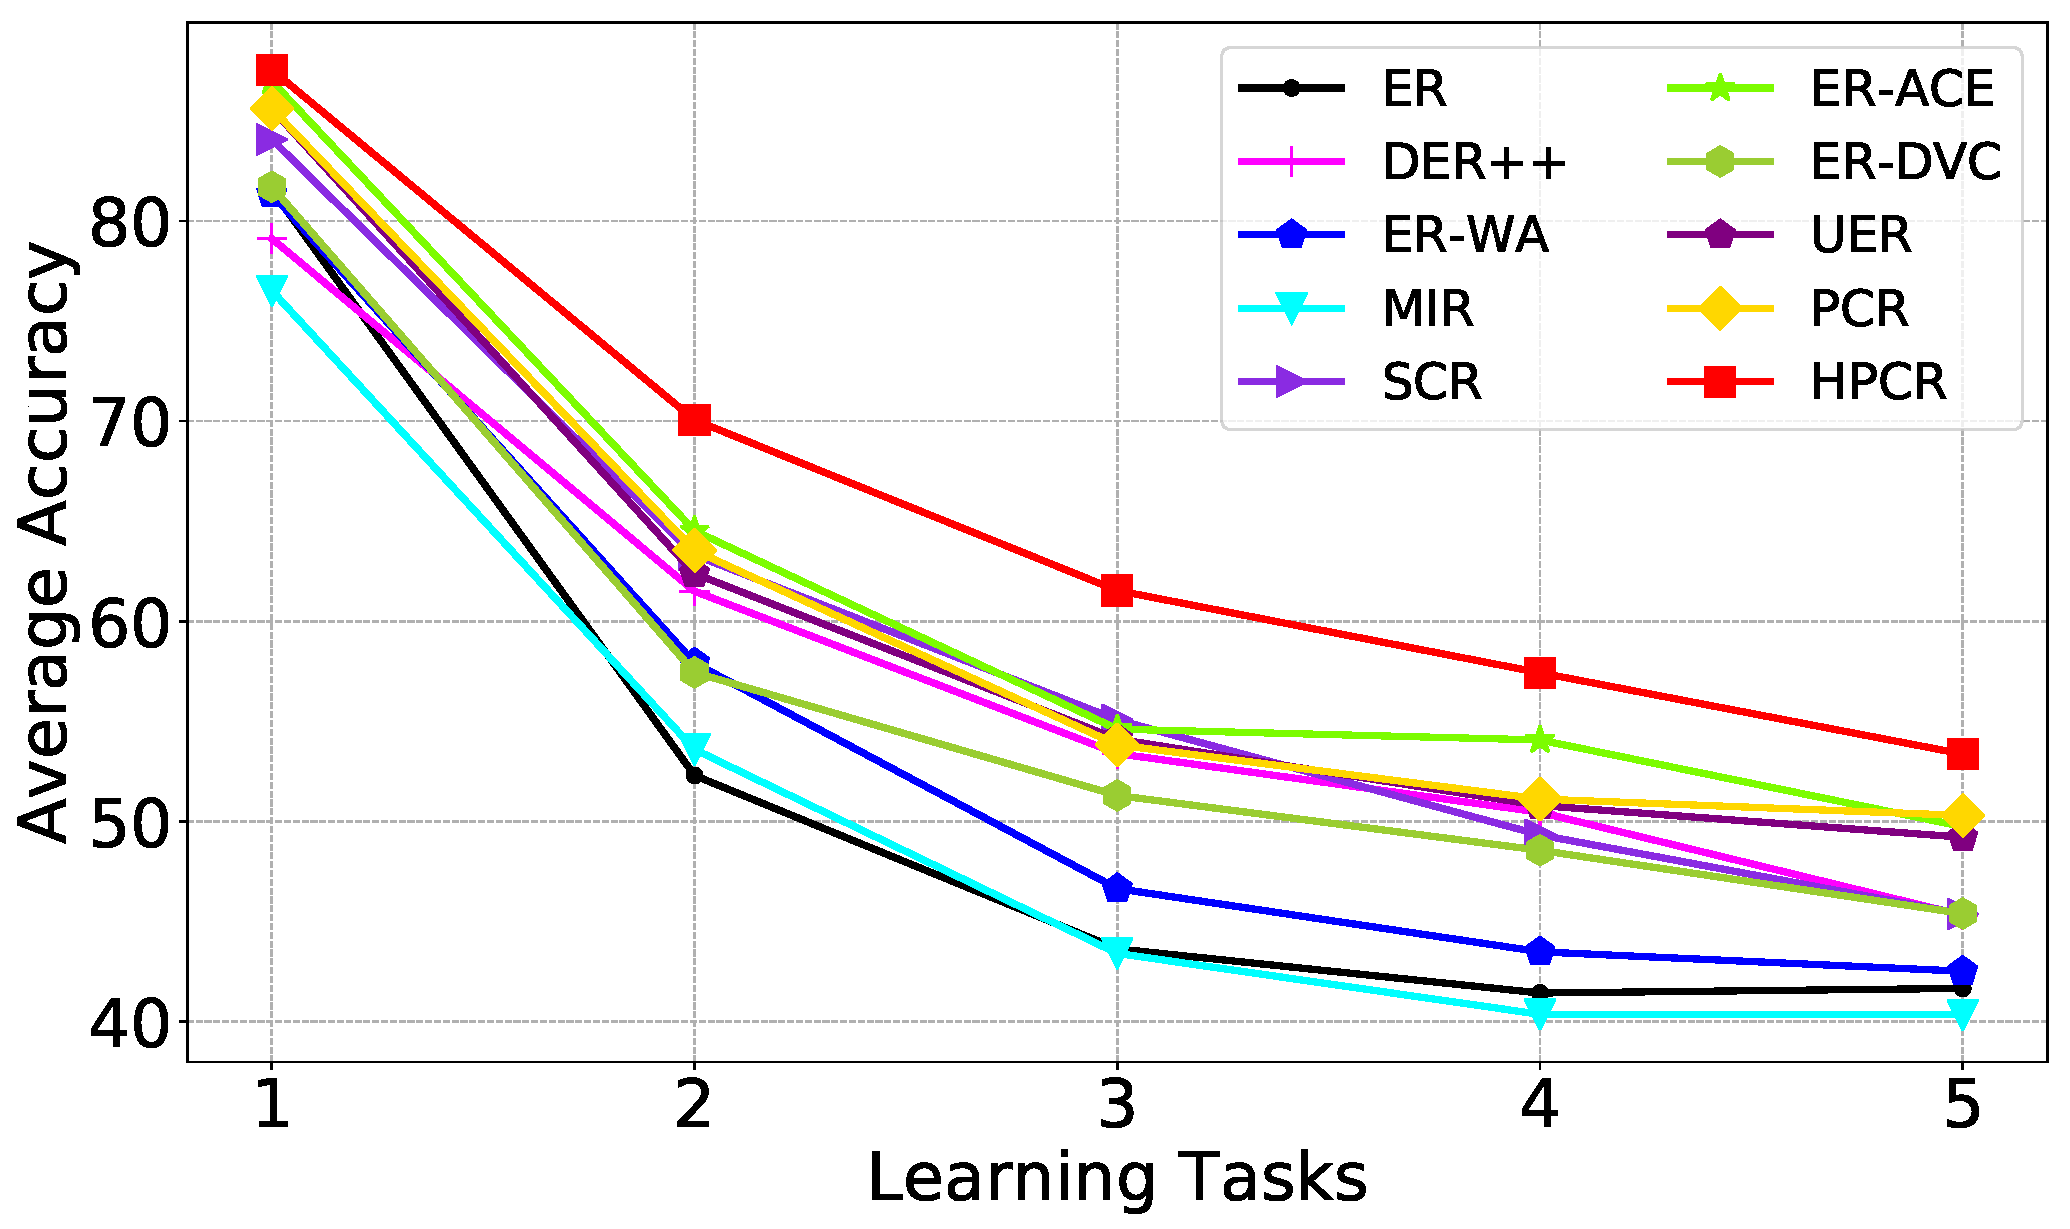
\includegraphics[scale=0.2]{sections/Figures/pcr_cifar10_acc_1000.pdf}
        {(a) Split CIFAR10 (Buffer=200)}
    \end{minipage}
    \begin{minipage}[t]{0.40\linewidth}
        \centering
        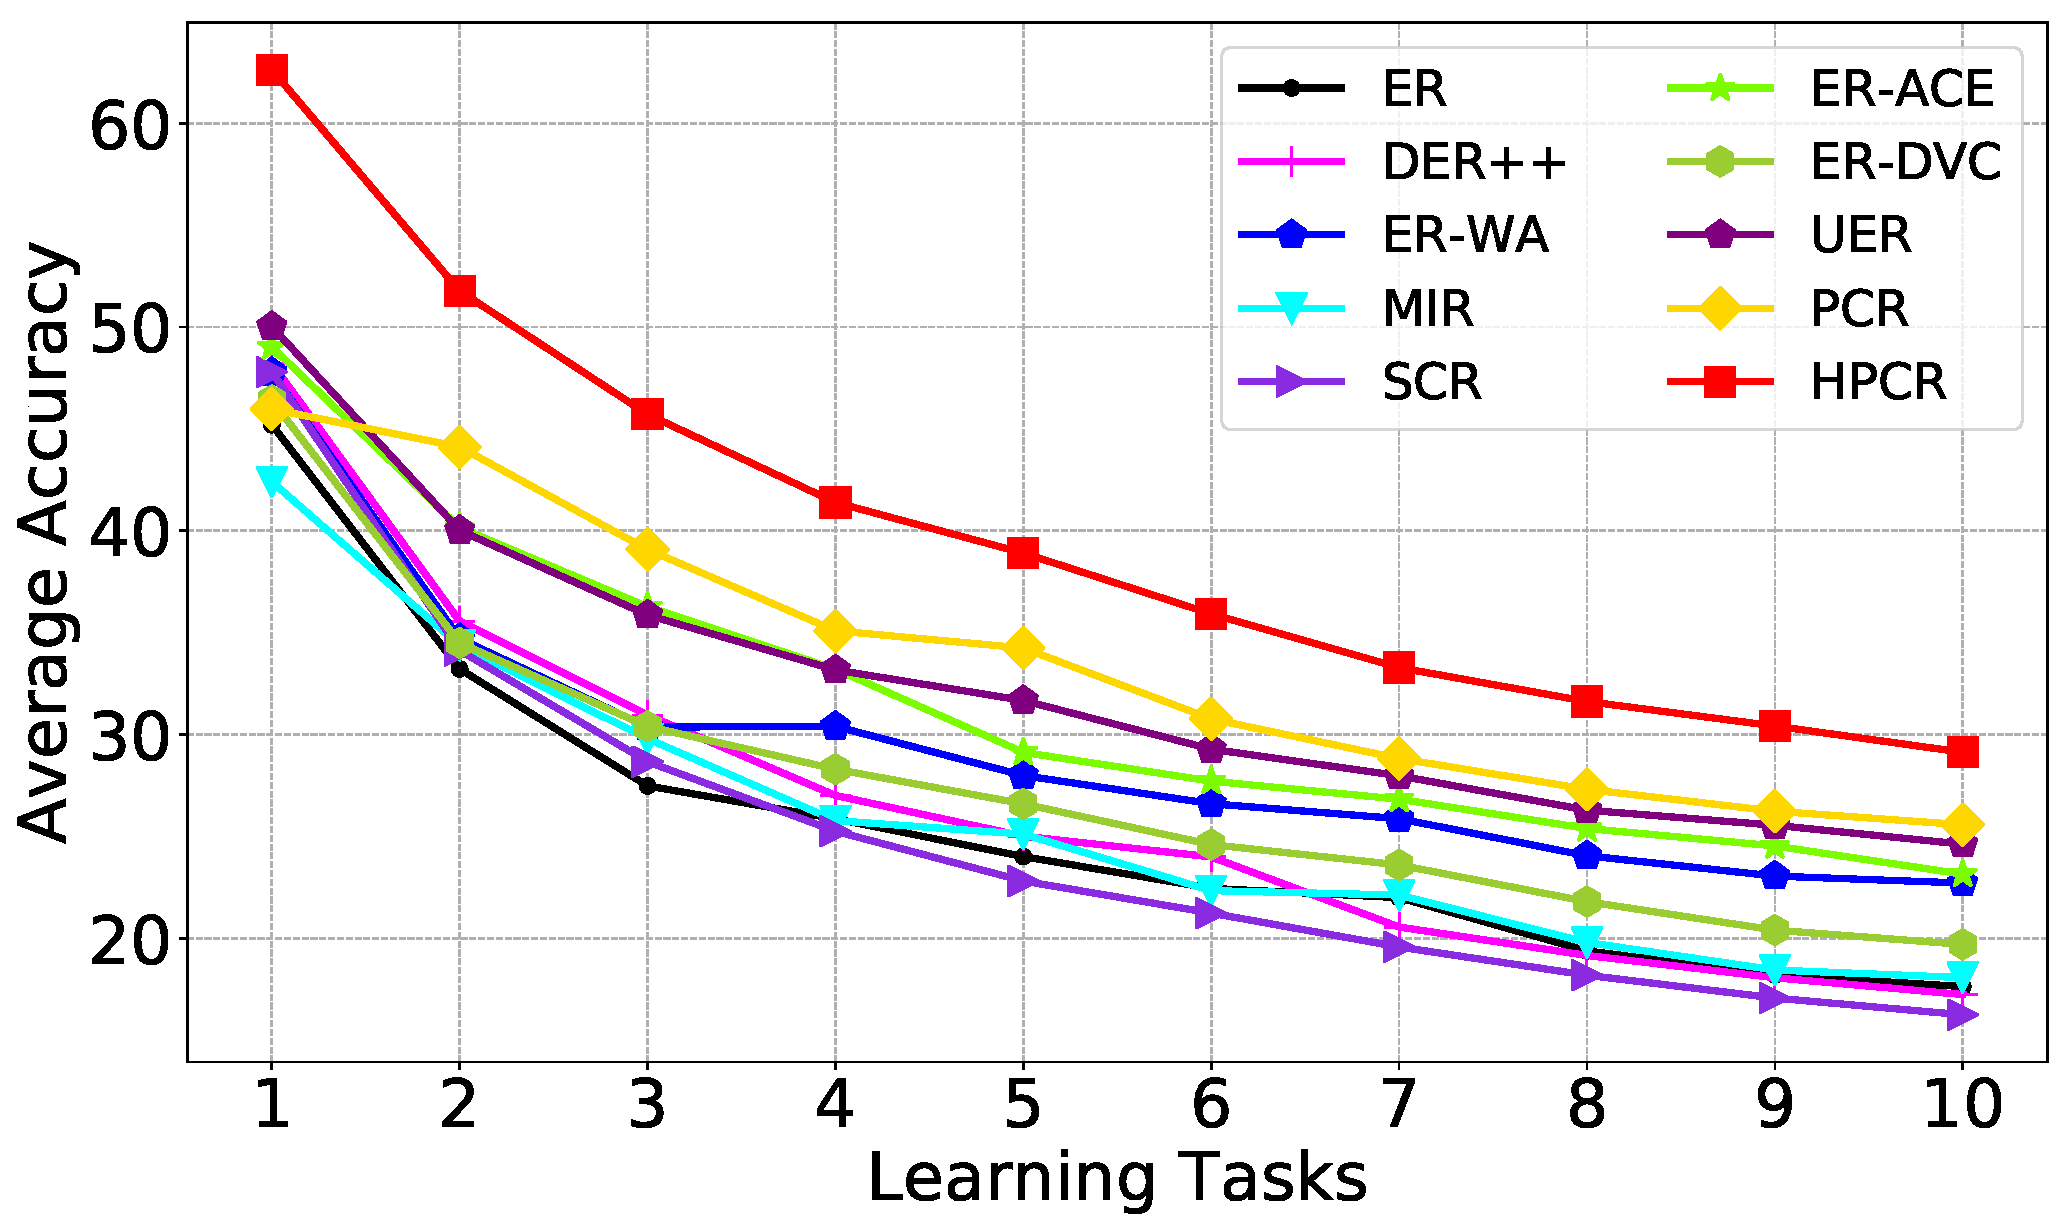
\includegraphics[scale=0.2]{sections/Figures/pcr_cifar100_acc_1000.pdf}
        {(b) Split CIFAR100 (Buffer=1000)}
    \end{minipage}
    \begin{minipage}[t]{0.40\linewidth}
        \centering
        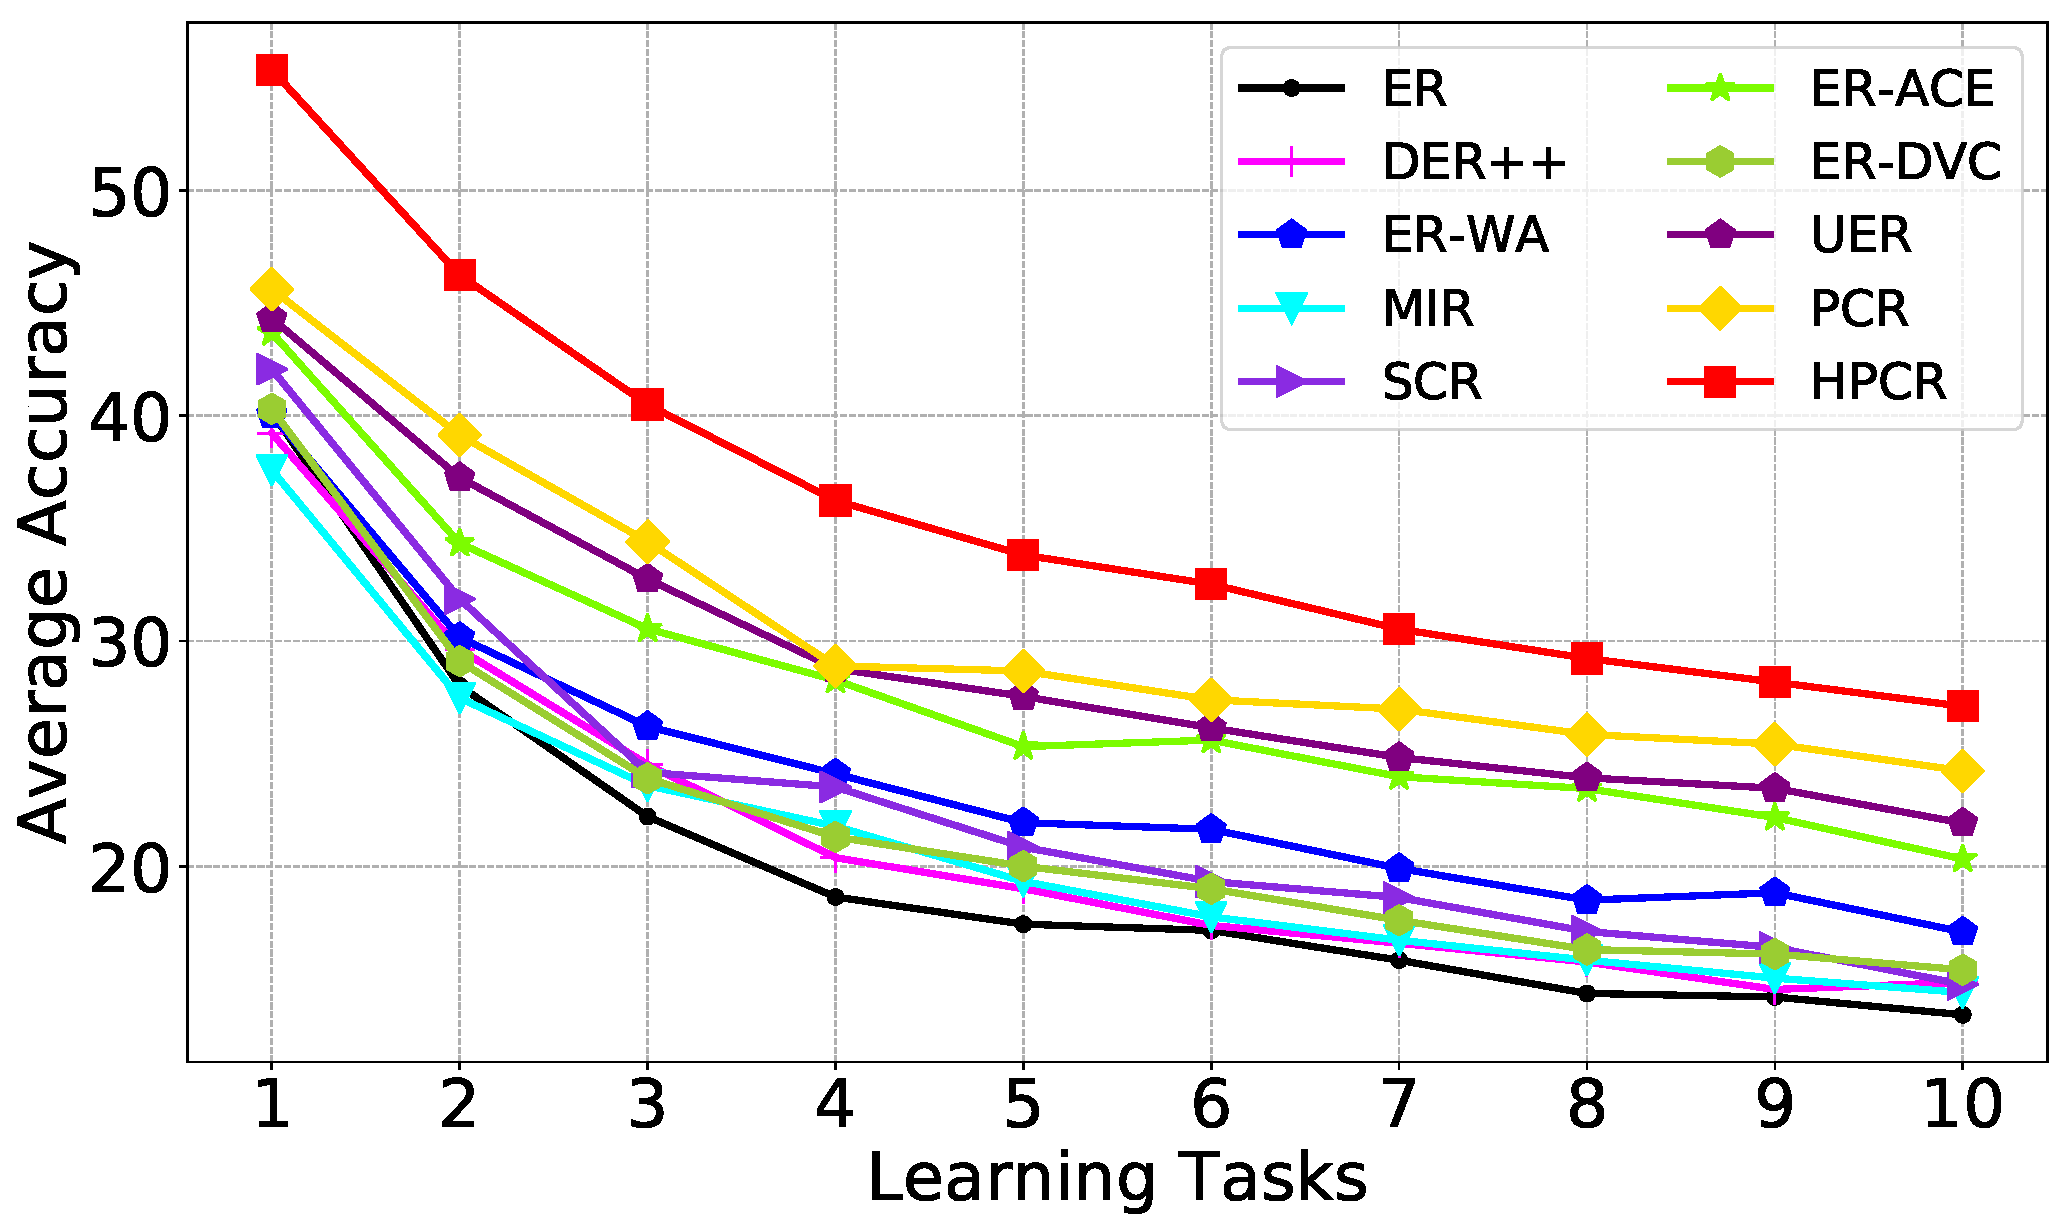
\includegraphics[scale=0.2]{sections/Figures/pcr_miniimagenet_acc_1000.pdf}
        {(c) Split MiniImageNet (Buffer=1000)}
    \end{minipage}
    \begin{minipage}[t]{0.40\linewidth}
        \centering
        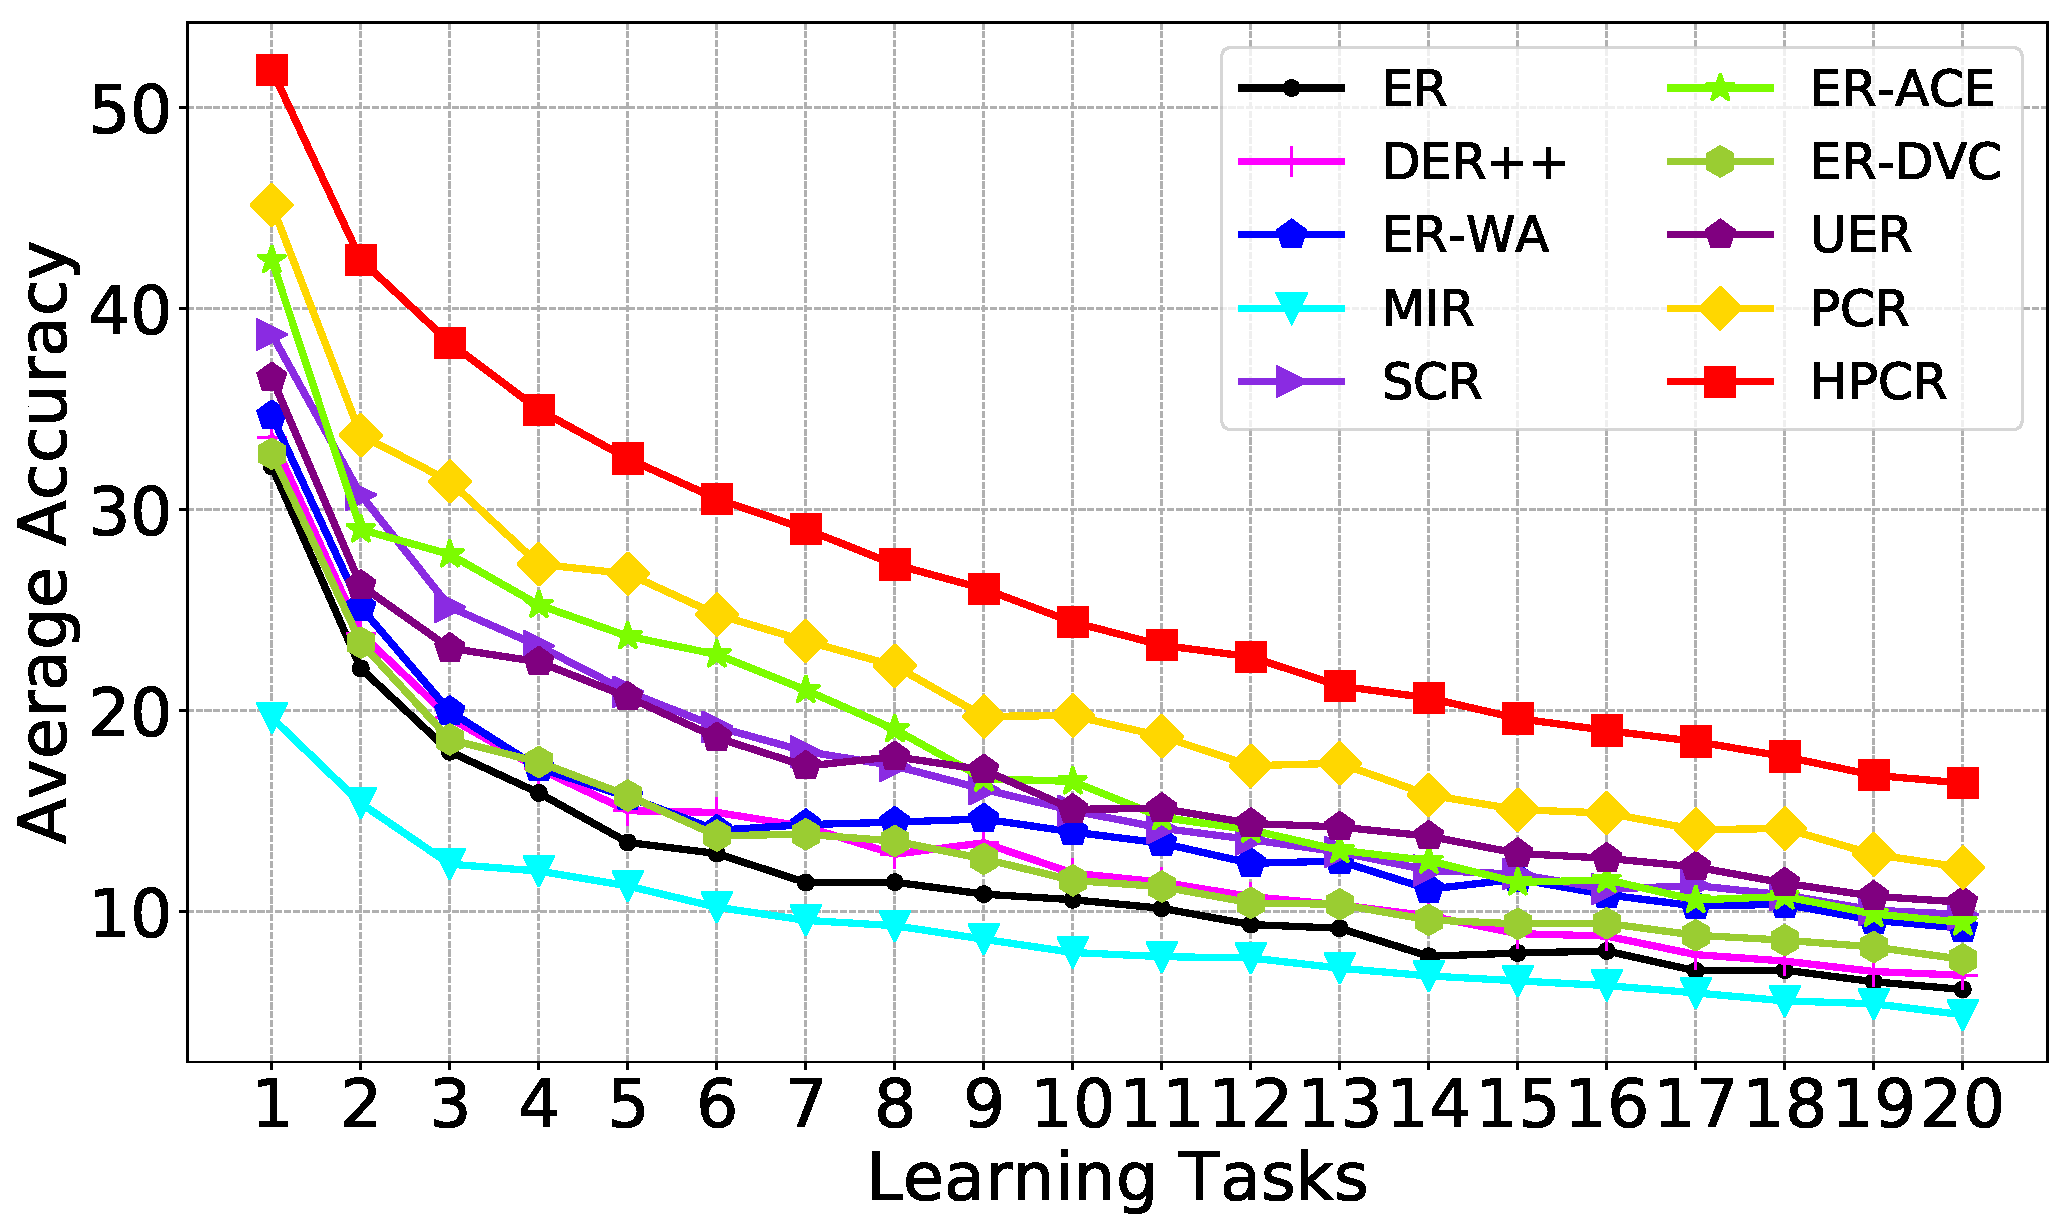
\includegraphics[scale=0.2]{sections/Figures/pcr_tinyimagenet_acc_1000.pdf}
        {(d) Split TinyImageNet (Buffer=2000)}
    \end{minipage}
\centering
\vspace{-1ex}
\caption{Average accuracy rate on observed learning tasks on all datasets. }
\label{learningstage1000}
\vspace{-2ex}
\end{figure*}

\begin{figure*}[t]
\centering
    \begin{minipage}[t]{0.4\linewidth}
        \centering
        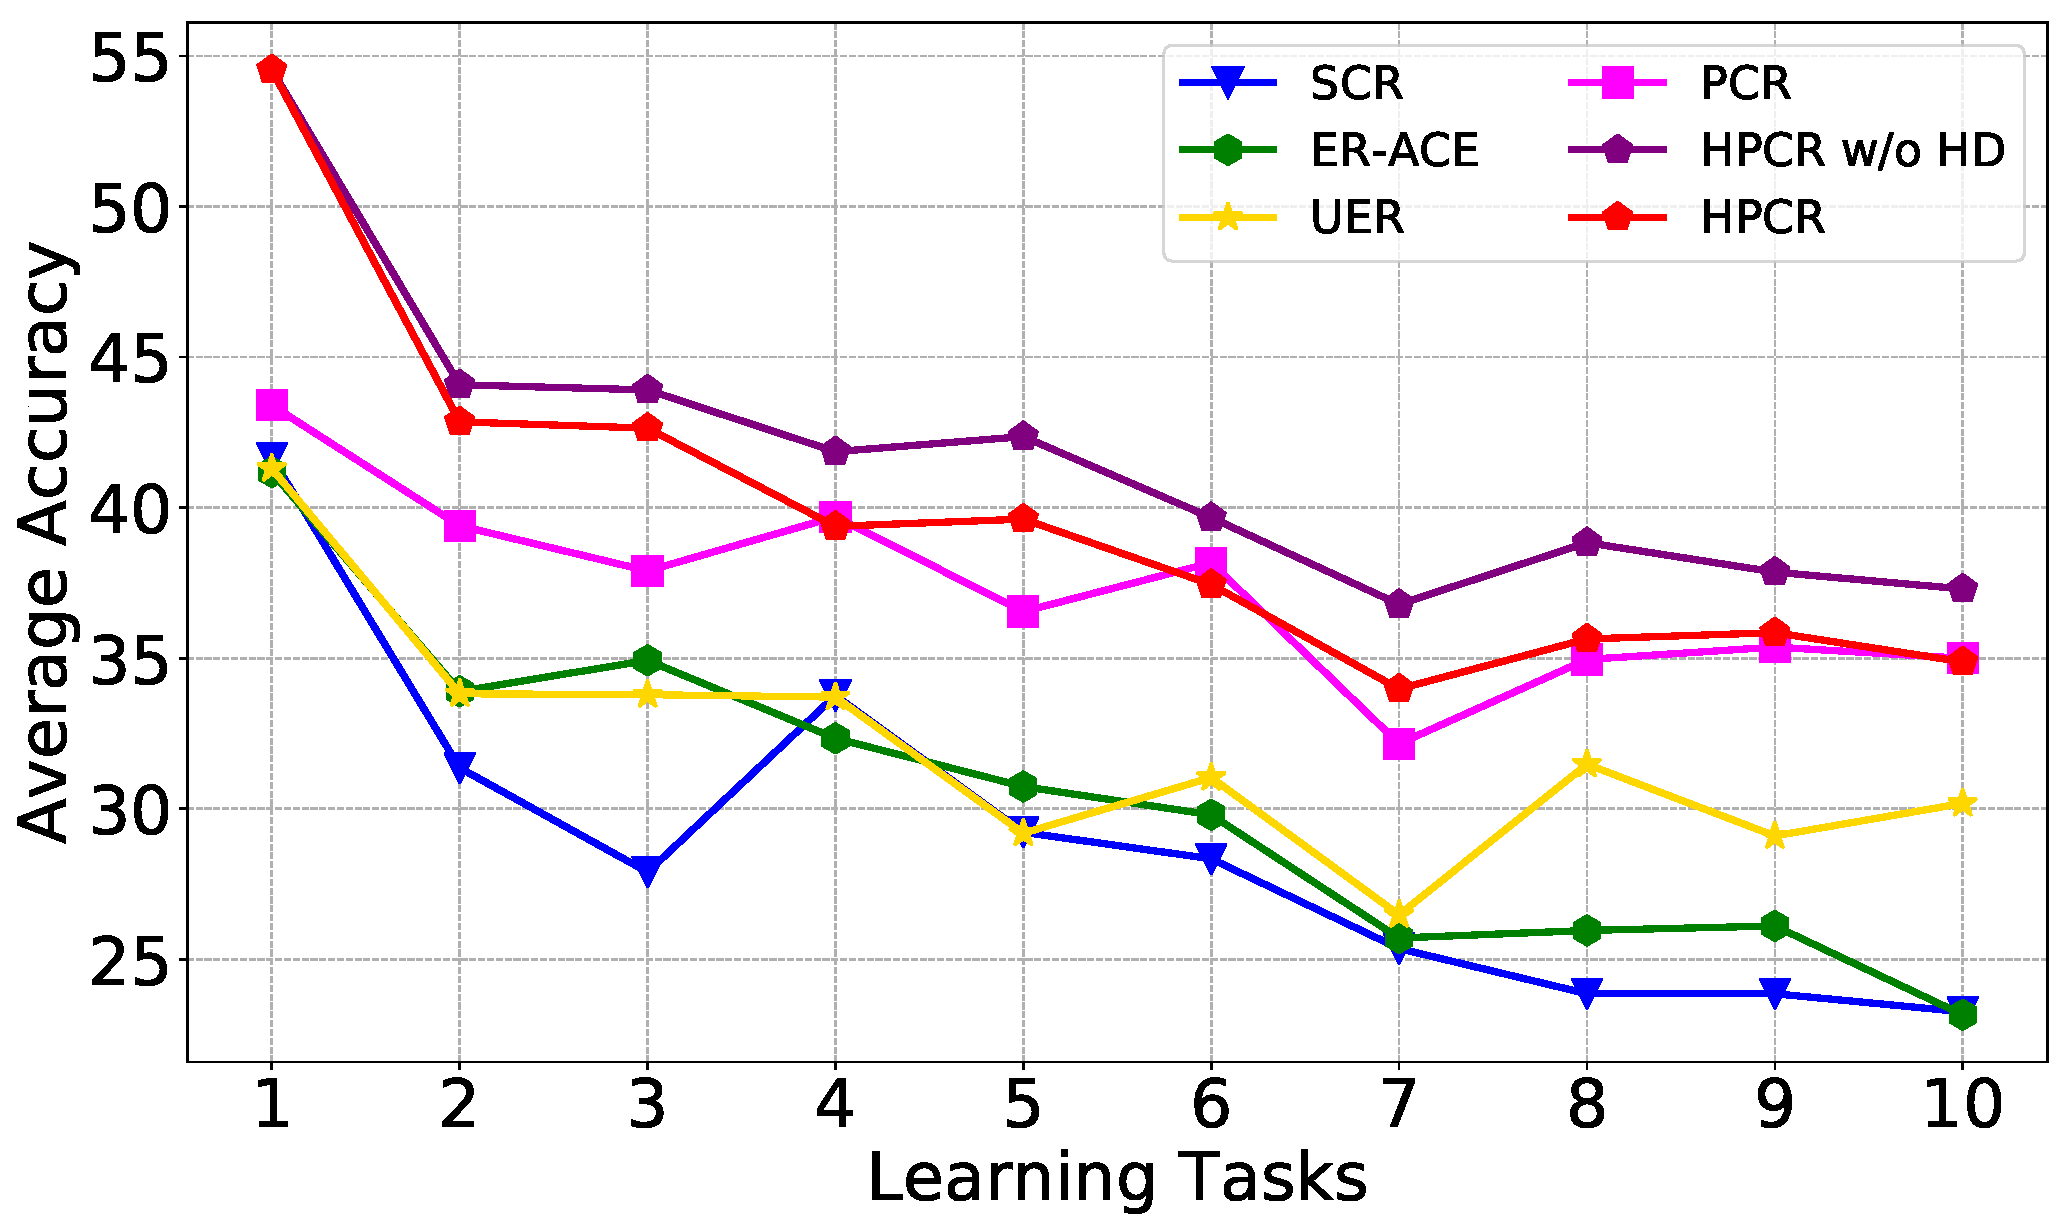
\includegraphics[scale=0.2]{sections/Figures/pcr_new_acc_1000.pdf}
        {(a) Performance on novel knowledge}
    \end{minipage}
    \begin{minipage}[t]{0.4\linewidth}
        \centering
        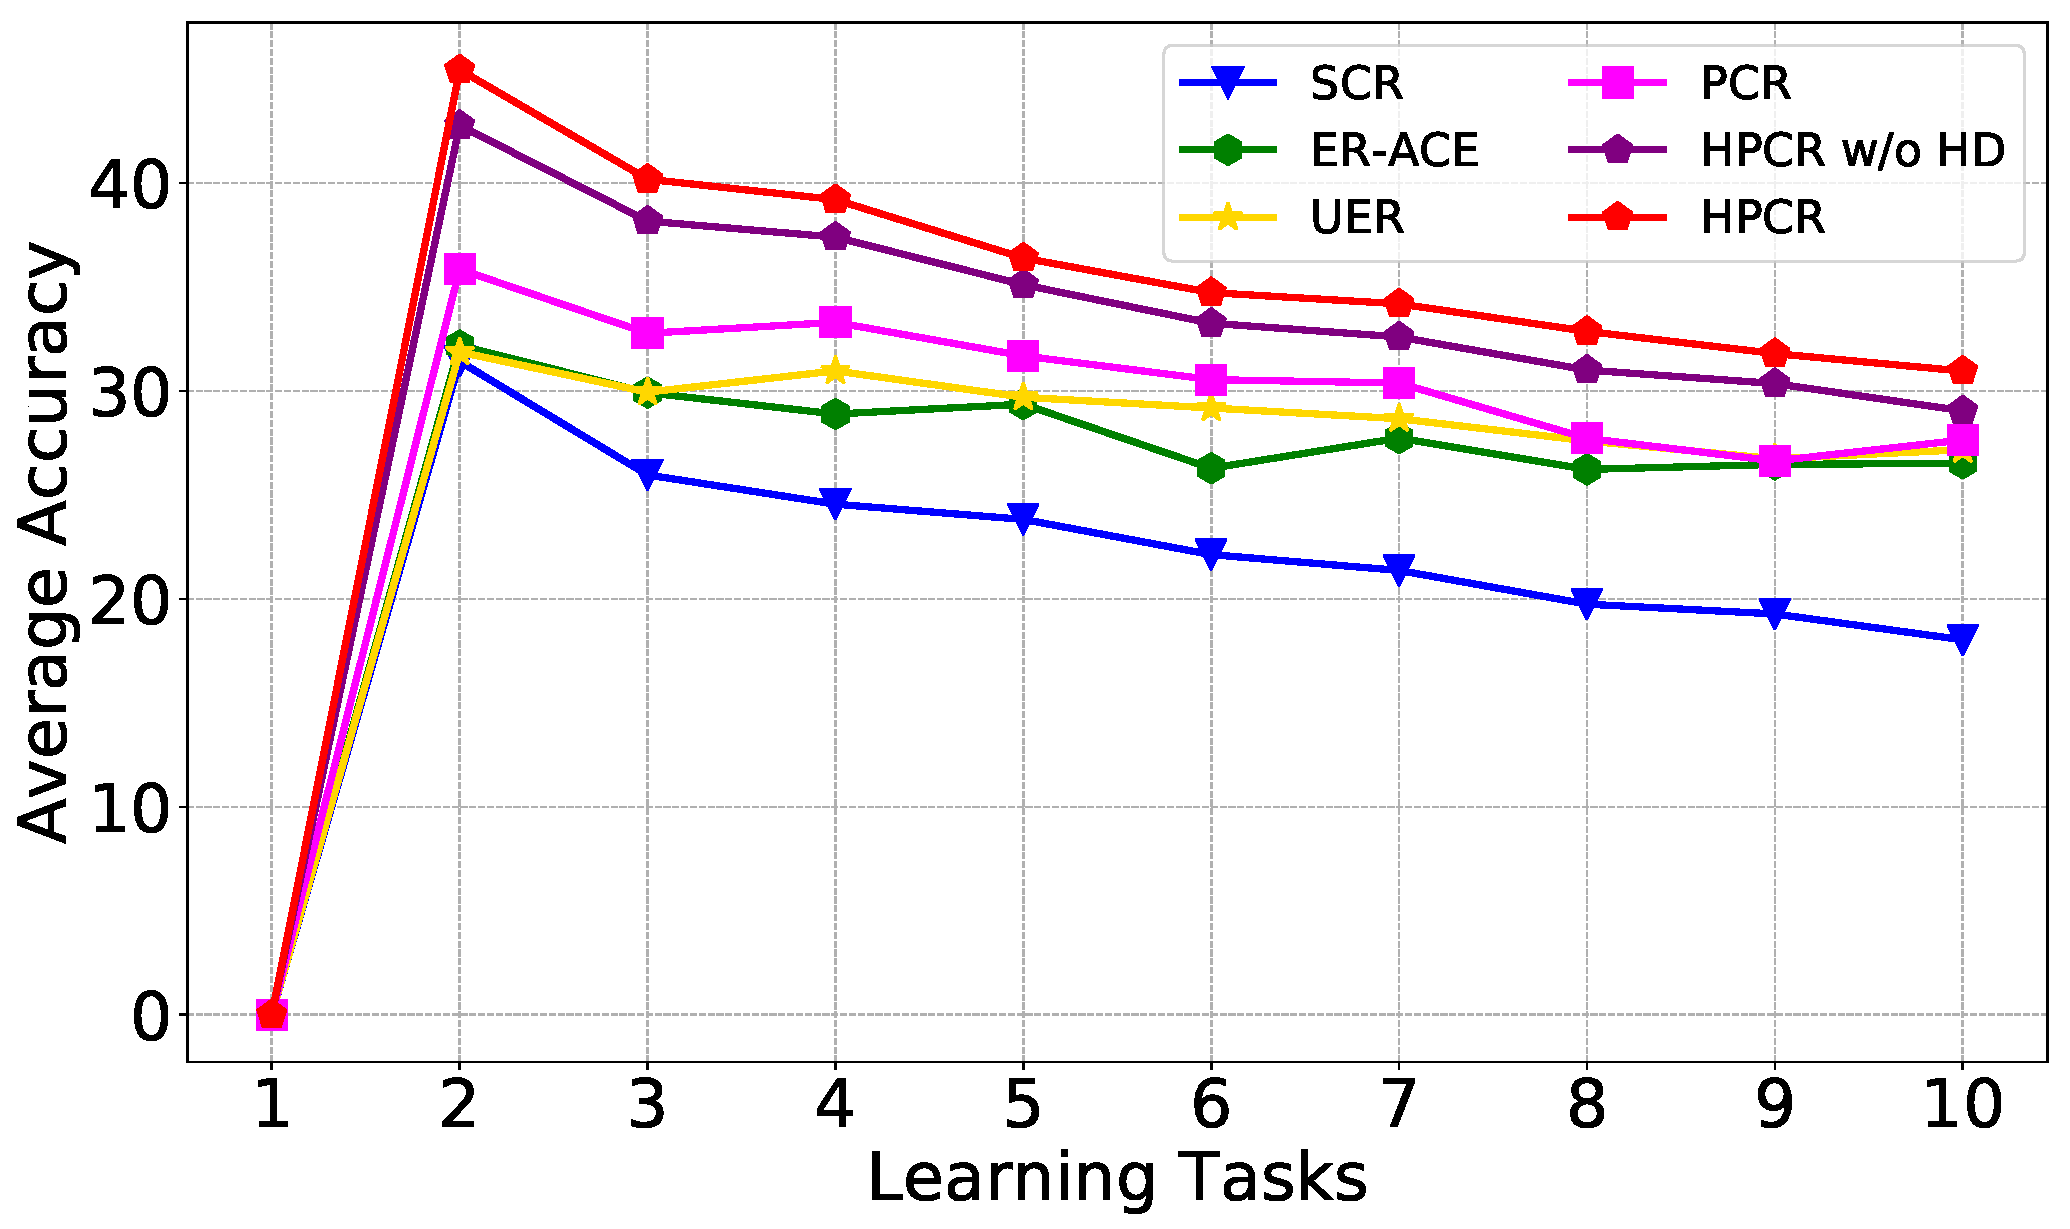
\includegraphics[scale=0.2]{sections/Figures/pcr_old_acc_1000.pdf}
        {(b) Performance on historical knowledge}
    \end{minipage}
\centering
\vspace{-1ex}
\caption{Average accuracy rate on observed learning tasks Split MiniImageNet while the buffer size is 5000. }
\label{learningstage5000}
\vspace{-2ex}
\end{figure*}

\begin{table*}[t]\small
\renewcommand\tabcolsep{2pt}
\centering
\caption{Final Forgetting Rate (↓) for four datasets.}
\vspace{-1ex}
\label{tableforget}
\begin{tabular}{l|ccc|ccc|ccc|ccc}
\hline
Datasets & \multicolumn{3}{c|}{Split CIFAR10 (\%)} & \multicolumn{3}{c|}{Split CIFAR100 (\%)}& \multicolumn{3}{c|}{Split MiniImageNet (\%)} & \multicolumn{3}{c}{Split TinyImageNet (\%)}\\ \hline
Buffer & \multicolumn{1}{c|}{100} & \multicolumn{1}{c|}{200} & \multicolumn{1}{c|}{500} & \multicolumn{1}{c|}{1000}    & \multicolumn{1}{c|}{2000} & \multicolumn{1}{c|}{5000} & \multicolumn{1}{c|}{1000} & \multicolumn{1}{c|}{2000}     &\multicolumn{1}{c|}{5000} & \multicolumn{1}{c|}{2000} & \multicolumn{1}{c|}{4000} & 10000     \\ \hline
SCR~\cite{mai2021supervised} (CVPR-W2021)   & 51.7\scriptsize±4.3 & 39.6\scriptsize±2.0                 & 27.7\scriptsize±2.9                 & 13.2\scriptsize±1.3                  & 12.9\scriptsize±1.5                  & 12.5\scriptsize±0.6 & 11.6\scriptsize±1.9                   & 11.5\scriptsize±1.4                  & 10.4\scriptsize±1.0 & 10.1\scriptsize±0.6                   & 8.7\scriptsize±0.6                  & 9.0\scriptsize±0.8\\
ER-ACE~\cite{caccia2021new} (ICLR2022)   & {18.7\scriptsize±1.1}& {17.1\scriptsize±2.5}                 & {13.8\scriptsize±1.7}                 & {10.5\scriptsize±0.8}                  & {9.8\scriptsize±0.5}                  & {7.9\scriptsize±1.5} & {9.8\scriptsize±1.1}                   & {7.3\scriptsize±1.4}                  & {6.2\scriptsize±0.9} & {9.2\scriptsize±0.9}                   & {7.5\scriptsize±0.4}                  & {6.4\scriptsize±0.7}\\
UER~\cite{lin2023uer} (ACMMM2023)   & {38.5\scriptsize±3.4}  & {30.7\scriptsize±3.6}  & {24.0\scriptsize±2.5}                 & {13.2\scriptsize±0.7}  & {9.8\scriptsize±1.0}  & {7.0\scriptsize±0.4} & {12.7\scriptsize±1.2}  & {8.4\scriptsize±0.7}  & {6.1\scriptsize±0.9} & 13.3\scriptsize±0.9                   & 9.0\scriptsize±1.0                  & 6.7\scriptsize±1.1\\
\hline

HPCR (Algorithm (\ref{alg:hpcr}))   & {28.5\scriptsize±1.2}& {20.6\scriptsize±2.4}                 & {15.5\scriptsize±1.8}                 & {15.7\scriptsize±0.7}                  & {11.1\scriptsize±0.5}                  & {9.3\scriptsize±0.8} & {15.4\scriptsize±0.6}                   & {11.1\scriptsize±0.7}                  & {8.6\scriptsize±0.4} & {20.5\scriptsize±0.8}                   & {13.6\scriptsize±1.1}                  & {9.2\scriptsize±0.7}\\
$\hookrightarrow$PCR   & 25.8\scriptsize±2.3& 19.4\scriptsize±3.3                 & 17.1\scriptsize±2.4                 & 15.5\scriptsize±0.9                  & 11.7\scriptsize±2.4                  & 9.5\scriptsize±0.8                  & 13.7\scriptsize±1.1 & 10.8\scriptsize±1.4                   & 9.5\scriptsize±1.5                  & 20.6\scriptsize±0.8 & 13.7\scriptsize±0.7                   & 10.2\scriptsize±0.6\\
\hline
\end{tabular}
\vspace{-4ex}
\end{table*}




\subsection{Overall Performance}
In this section, we conduct experiments to compare with various state-of-the-art baselines. The overall performance of PCR is advanced compared to all baselines. Moreover, HPCR obtains significantly improved performance on four datasets.

\textbf{Comparison on final accuracy.} HPCR has consistently achieved the best performance compared to all baseline methods. 
Table~\ref{tableaccuracy} shows the final accuracy rate for all datasets. All reported scores are the average score of 10 runs with 95\%
confidence interval. In a multitude of experimental scenarios, where each dataset comprises four memory buffers of varying sizes, HPCR consistently outshines all other methods. In particular, it exhibits even more remarkable performance compared to PCR. Specifically, HPCR shows a significant advancement, incorporating contrastive, temperature, and distillation components to further refine the PCR framework. For instance, on Split Cifar10, HPCR outperforms PCR by noteworthy margins of 2.9\%, 3.1\%, and 4.1\% for memory buffer sizes of 100, 200, and 500, respectively. These compelling results unequivocally highlight the crucial significance of the components introduced in this article, as they play a pivotal role in elevating the performance of PCR. 


Moreover, we conduct a comprehensive comparative analysis between five methods, utilizing the experimental setup outlined in \cite{guo2022online}. In this particular study, the model is configured as ResNet18 with 64 filters, and 64 samples are retrieved from the memory buffer for each training batch. The training process employs the Adam optimizer with a learning rate 0.001. It is important to note that these experimental conditions differ from those employed in our own study. As presented in Table~\ref{moreaccuracy}, HPCR demonstrates remarkable superiority over SCR, OCM, OnPro, and PCR under different experimental settings. This evidence further reinforces the effectiveness and robustness of HPCR in comparison to existing approaches.

\begin{table*}[t]\small
\renewcommand\tabcolsep{2pt}
\centering
\caption{Final Accuracy Rate (higher is better) for ablation studies. ER acts as a baseline method.}
\vspace{-1ex}
\label{ablation}
\begin{tabular}{l|ccc|ccc|ccc|ccc}
\hline
Datasets & \multicolumn{3}{c|}{Split CIFAR10} & \multicolumn{3}{c|}{Split CIFAR100}& \multicolumn{3}{c|}{Split MiniImageNet}& \multicolumn{3}{c}{Split TinyImageNet}\\ \hline
Buffer & \multicolumn{1}{c|}{100} & \multicolumn{1}{c|}{200} & \multicolumn{1}{c|}{500} & \multicolumn{1}{c|}{1000} & \multicolumn{1}{c|}{2000} & \multicolumn{1}{c|}{5000}     & \multicolumn{1}{c|}{1000} & \multicolumn{1}{c|}{2000} & \multicolumn{1}{c|}{5000} & \multicolumn{1}{c|}{2000} & \multicolumn{1}{c|}{4000} & 10000     \\ \hline
ER & 33.8\scriptsize±3.2& 41.7\scriptsize±2.8                 & 46.0\scriptsize±3.5                 & 17.6\scriptsize±0.9                  & 19.7\scriptsize±1.6                  & 20.9\scriptsize±1.2 & 13.4\scriptsize±0.9                   & 16.5\scriptsize±0.9                  & 16.2\scriptsize±1.7                  & 6.1\scriptsize±0.5                  & 8.5\scriptsize±0.7                  & 8.9\scriptsize±0.6\\
Couple (Equation~(\ref{eq:coupleloss1})) & 38.4\scriptsize±3.0& 43.2\scriptsize±3.8                 & 49.1\scriptsize±3.9                 & 179\scriptsize±0.8                  & 19.7\scriptsize±0.8                  & 21.6\scriptsize±1.0 & 17.9\scriptsize±0.7                   & 19.9\scriptsize±0.8                  & 20.9\scriptsize±1.6                  & 5.2\scriptsize±0.4                  & 10.7\scriptsize±0.7                  & 12.8\scriptsize±0.5\\
Couple (Equation~(\ref{eq:coupleloss2})) & 34.1\scriptsize±2.3& 41.8\scriptsize±3.9                 & 46.3\scriptsize±2.8                 & 18.7\scriptsize±0.9                  & 20.7\scriptsize±0.8                  & 21.8\scriptsize±0.9 & 16.3\scriptsize±0.8                   & 18.7\scriptsize±0.7                  & 19.8\scriptsize±0.9                  & 6.2\scriptsize±0.3                  & 10.1\scriptsize±0.6                  & 11.0\scriptsize±0.8\\
PCR    & 45.4\scriptsize±1.3& 50.3\scriptsize±1.5                & 56.0\scriptsize±1.2                 & 25.6\scriptsize±0.6                &27.4\scriptsize±0.6                 & 29.3\scriptsize±1.1 & 24.2\scriptsize±0.9                   & 27.2\scriptsize±1.2                  & 28.4\scriptsize±0.9                   & 12.2\scriptsize±0.9                   & 17.4\scriptsize±0.7                  & 19.6\scriptsize±0.8\\\hline
% ER+PS   & 39.4\scriptsize±3.2& 48.8\scriptsize±1.1                & 52.3\scriptsize±1.7                 & 25.5\scriptsize±0.6                &26.0\scriptsize±0.7                  & 28.2\scriptsize±0.7 & 22.8\scriptsize±0.8                   & 25.6\scriptsize±1.1                  & 27.5\scriptsize±1.0                   & 11.7\scriptsize±0.8                  & 15.7\scriptsize±1.1                  & 18.5\scriptsize±0.7\\

% ER+PS+PD (PCR)    & 45.4\scriptsize±1.3& 50.3\scriptsize±1.5                & 56.0\scriptsize±1.2                 & 25.6\scriptsize±0.6                &27.4\scriptsize±0.6                 & 29.3\scriptsize±1.1 & 24.2\scriptsize±0.9                   & 27.2\scriptsize±1.2                  & 28.4\scriptsize±0.9                   & 12.2\scriptsize±0.9                   & 17.4\scriptsize±0.7                  & 19.6\scriptsize±0.8\\
% ER+PS+PD+PC    & 43.7\scriptsize±1.2& 49.1\scriptsize±1.3                & 56.2\scriptsize±1.2                 & 26.0\scriptsize±0.4           & 28.2\scriptsize±0.6          & 30.1\scriptsize±1.0 & 23.5\scriptsize±0.6                   & 26.8\scriptsize±0.5                  & 28.0\scriptsize±0.6                   & 13.0\scriptsize±0.4                  & 17.2\scriptsize±0.4                  & 19.5\scriptsize±0.6\\\hline
PCR+HC ($\rm PCR_C$)    & 41.9\scriptsize±2.0& 48.3\scriptsize±2.4                & 55.8\scriptsize±1.2                 & 24.1\scriptsize±0.5           & 25.9\scriptsize±0.5          & 27.3\scriptsize±0.7 & 21.8\scriptsize±0.8                   & 24.5\scriptsize±0.9                  & 26.3\scriptsize±1.0                   & {11.1\scriptsize±1.2}                   & {13.6\scriptsize±0.7}                  & {15.3\scriptsize±1.2}\\

PCR+HC+HT ($\rm PCR_{CT}$)    & {47.4\scriptsize±2.2}& {51.3\scriptsize±1.6}                & {57.7\scriptsize±1.1}                 & {27.2\scriptsize±0.5}                &{29.3\scriptsize±0.7}                 & {31.6\scriptsize±0.9} & {25.6\scriptsize±1.0}                   & {28.5\scriptsize±0.5}                  & {29.8\scriptsize±0.7} & {14.8\scriptsize±0.6}                   & {18.8\scriptsize±0.5}                  & {20.8\scriptsize±0.5}\\
$\rm PCR_{CT}$+PCD    & 48.0\scriptsize±1.9& 52.4\scriptsize±1.2                & 59.1\scriptsize±1.2                 & 28.6\scriptsize±0.8           & 30.1\scriptsize±0.7          & 33.0\scriptsize±0.5 & 26.6\scriptsize±0.5                   & 29.3\scriptsize±0.6                  & 30.9\scriptsize±0.7                   & 15.6\scriptsize±0.3                  & 19.2\scriptsize±0.5                  & 21.8\scriptsize±0.6\\
$\rm PCR_{CT}$+PCD+SCD (HPCR)    & \textbf{48.3\scriptsize±1.5}& \textbf{53.4\scriptsize±1.4}                & \textbf{60.1\scriptsize±1.1}                 & \textbf{29.1\scriptsize±0.7}                &\textbf{30.7\scriptsize±0.5}                 & \textbf{33.7\scriptsize±0.6} & \textbf{27.1\scriptsize±0.6}                   & \textbf{29.9\scriptsize±0.7}                  & \textbf{31.3\scriptsize±0.7} & \textbf{16.4\scriptsize±0.3}                   & \textbf{19.5\scriptsize±0.8}                  & \textbf{22.1\scriptsize±0.5}\\
\hline
\end{tabular}
\vspace{-3ex}
\end{table*}



\textbf{Comparison on learning process.} In the meantime, HPCR performs the best overall throughout the entire learning process. Specifically, we report the averaged anytime accuracy for all datasets in Table~\ref{tableaaa}. The experimental results show that HPCR consistently outperforms other baselines during the whole learning process. For a more detailed comparison, we also report the accuracy of each learning task in Figure~\ref{learningstage1000}, which can further validate the overall performance of the methods. The results show that the performance of PCR in the first few tasks does not outperform other baselines. However, its improvement becomes more and more visible as the number of tasks increases, proving its power to overcome CF. For instance, PCR does not perform best in the first task, but it demonstrates outstanding advantages in the remaining tasks on Split CIFAR100. Fortunately, this issue has been resolved in HPCR. The comparison of the red and orange lines shows that HPCR still performs well in the first few tasks. Therefore, our approaches have a stronger ability to resist forgetting.

\textbf{Comparison on knowledge balance.} Finally, HPCR also has significant advantages in balancing historical and novel knowledge. Before this, we calculate the final forgetting rate of the model when using different methods. As reported in Table~\ref{tableforget}, the existing methods, especially ER-ACE, have shown outstanding performance in this evaluation metric.
This is because ER-ACE tends to learn less, making it easily forget less. To verify it, we record the accuracy of novel and historical knowledge in each task for part of effective methods on Split MiniImageNet. As demonstrated in Figure~\ref{learningstage5000}, as ER-ACE learns less novel knowledge, its performance on the final forgetting rate can be better.

Actually, we should not only focus on the model's ability to retain historical knowledge, but also ensure the model's ability to quickly learn novel knowledge. Although SCR, ER-ACE, and UER can improve the anti-forgetting ability of the model, they tend to limit the generalization ability of the model. As the historical knowledge is consolidated, the learning performance of the model on novel knowledge becomes very poor. Different from existing studies, our model can not only effectively alleviate the phenomenon of CF, but also reduce the decline of the model at the generalization level as much as possible. Compared with HPCR (red line) and PCR (orange line), it is not difficult to find that there is a significant improvement in the memory ability of old knowledge.

\begin{figure}[t]
\centering
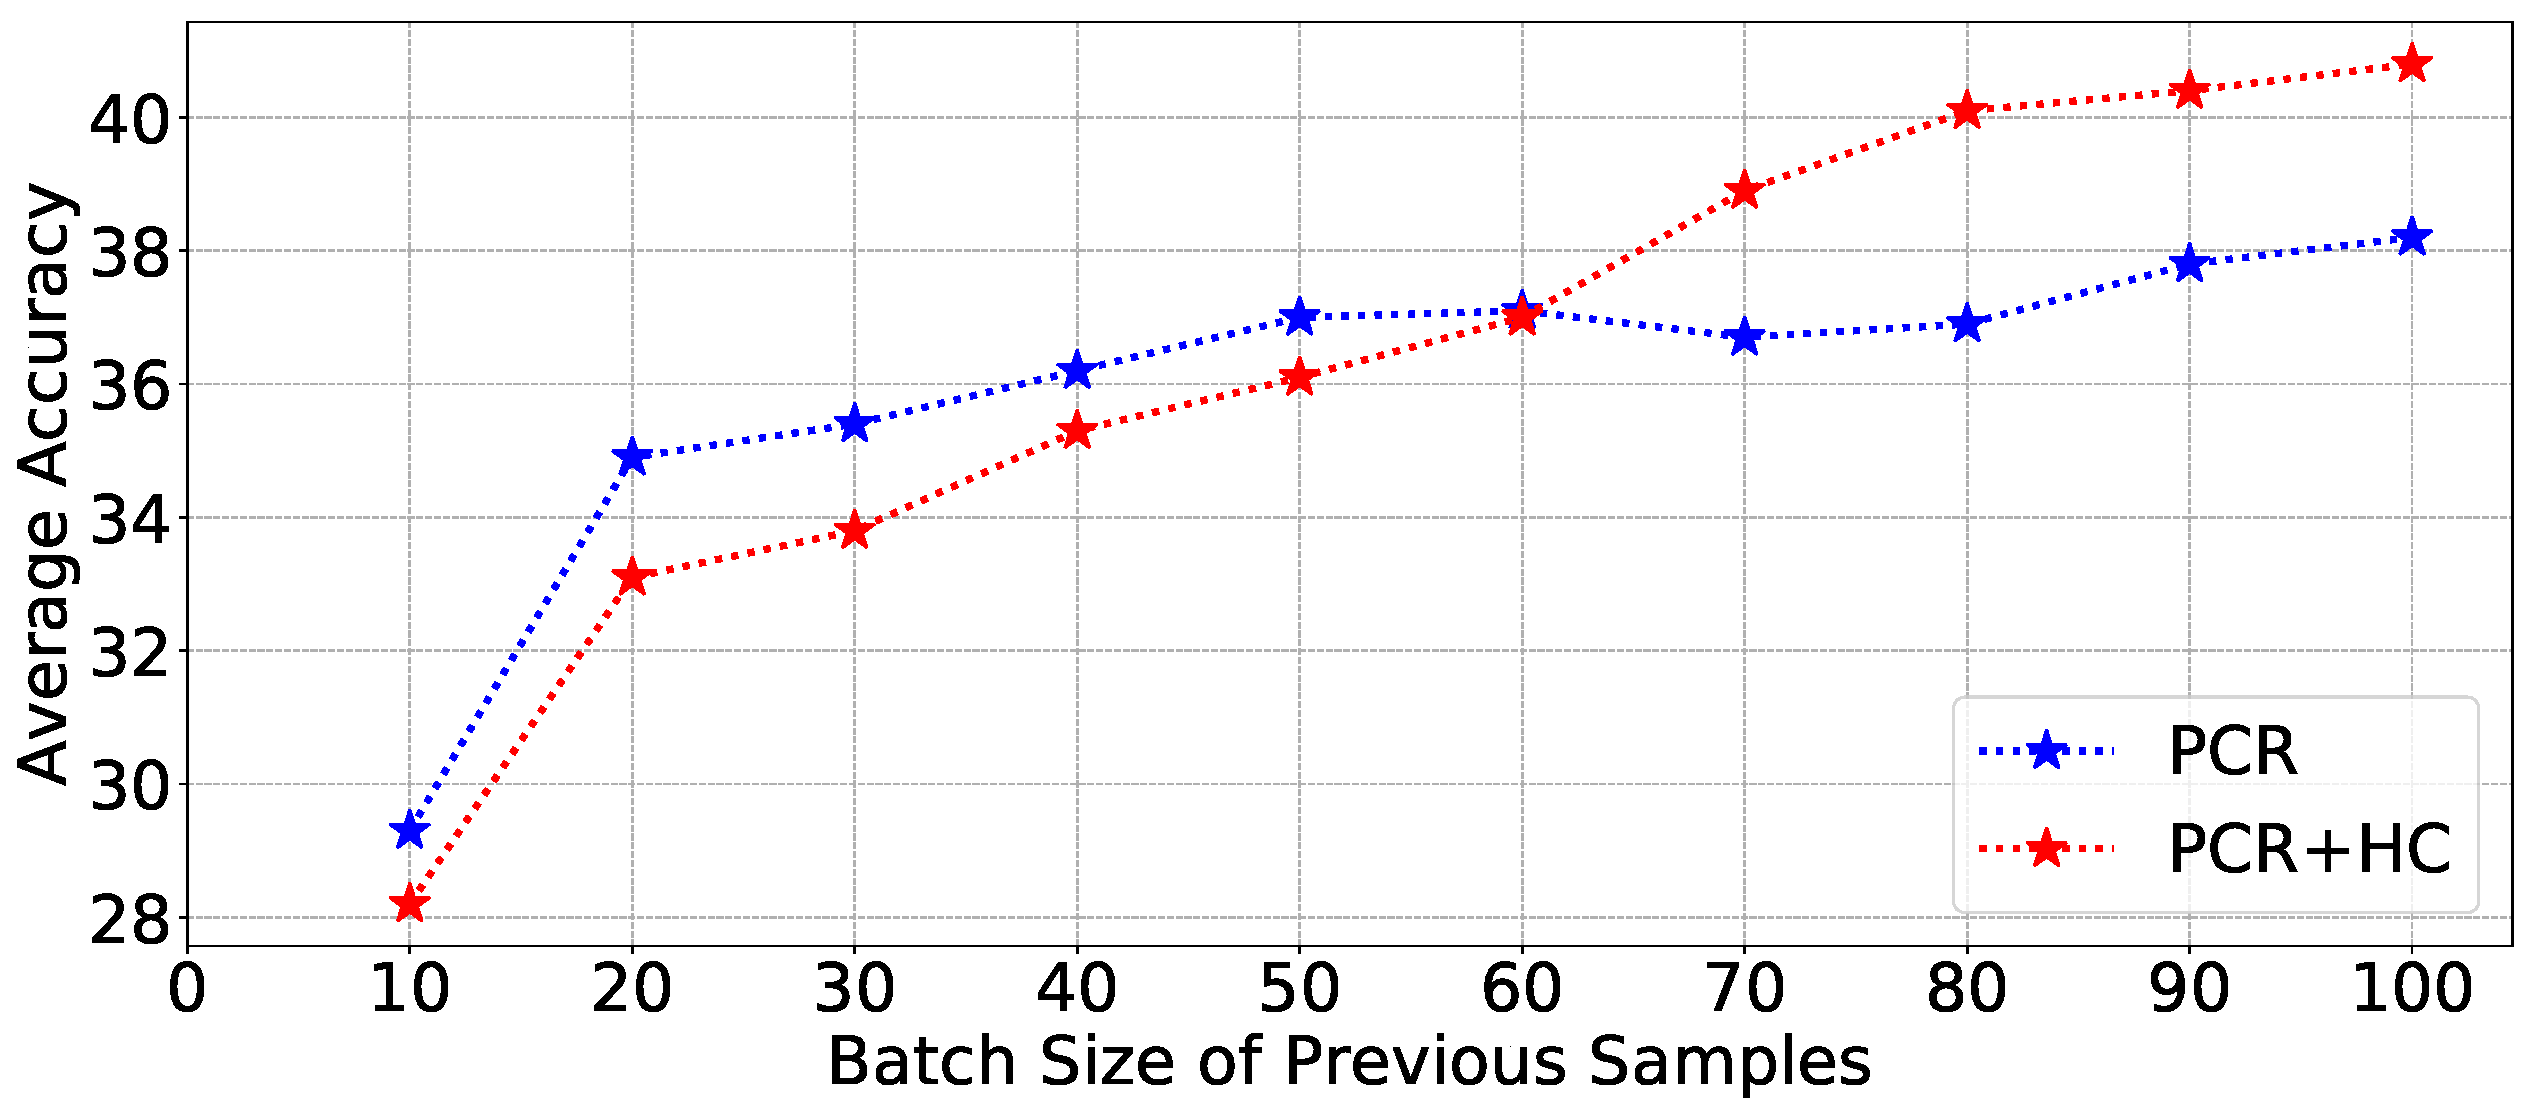
\includegraphics[scale=0.18]{sections/Figures/pcr_cifar100_hc.pdf}
\vspace{-2ex}
\caption{Final Accuracy Rate on Split CIFAR100 (buffer size=5000) with different batch sizes of previous samples.}
\label{fig:ablation_hc}%
\vspace{-2ex}
\end{figure}

\begin{figure}[t]
\centering
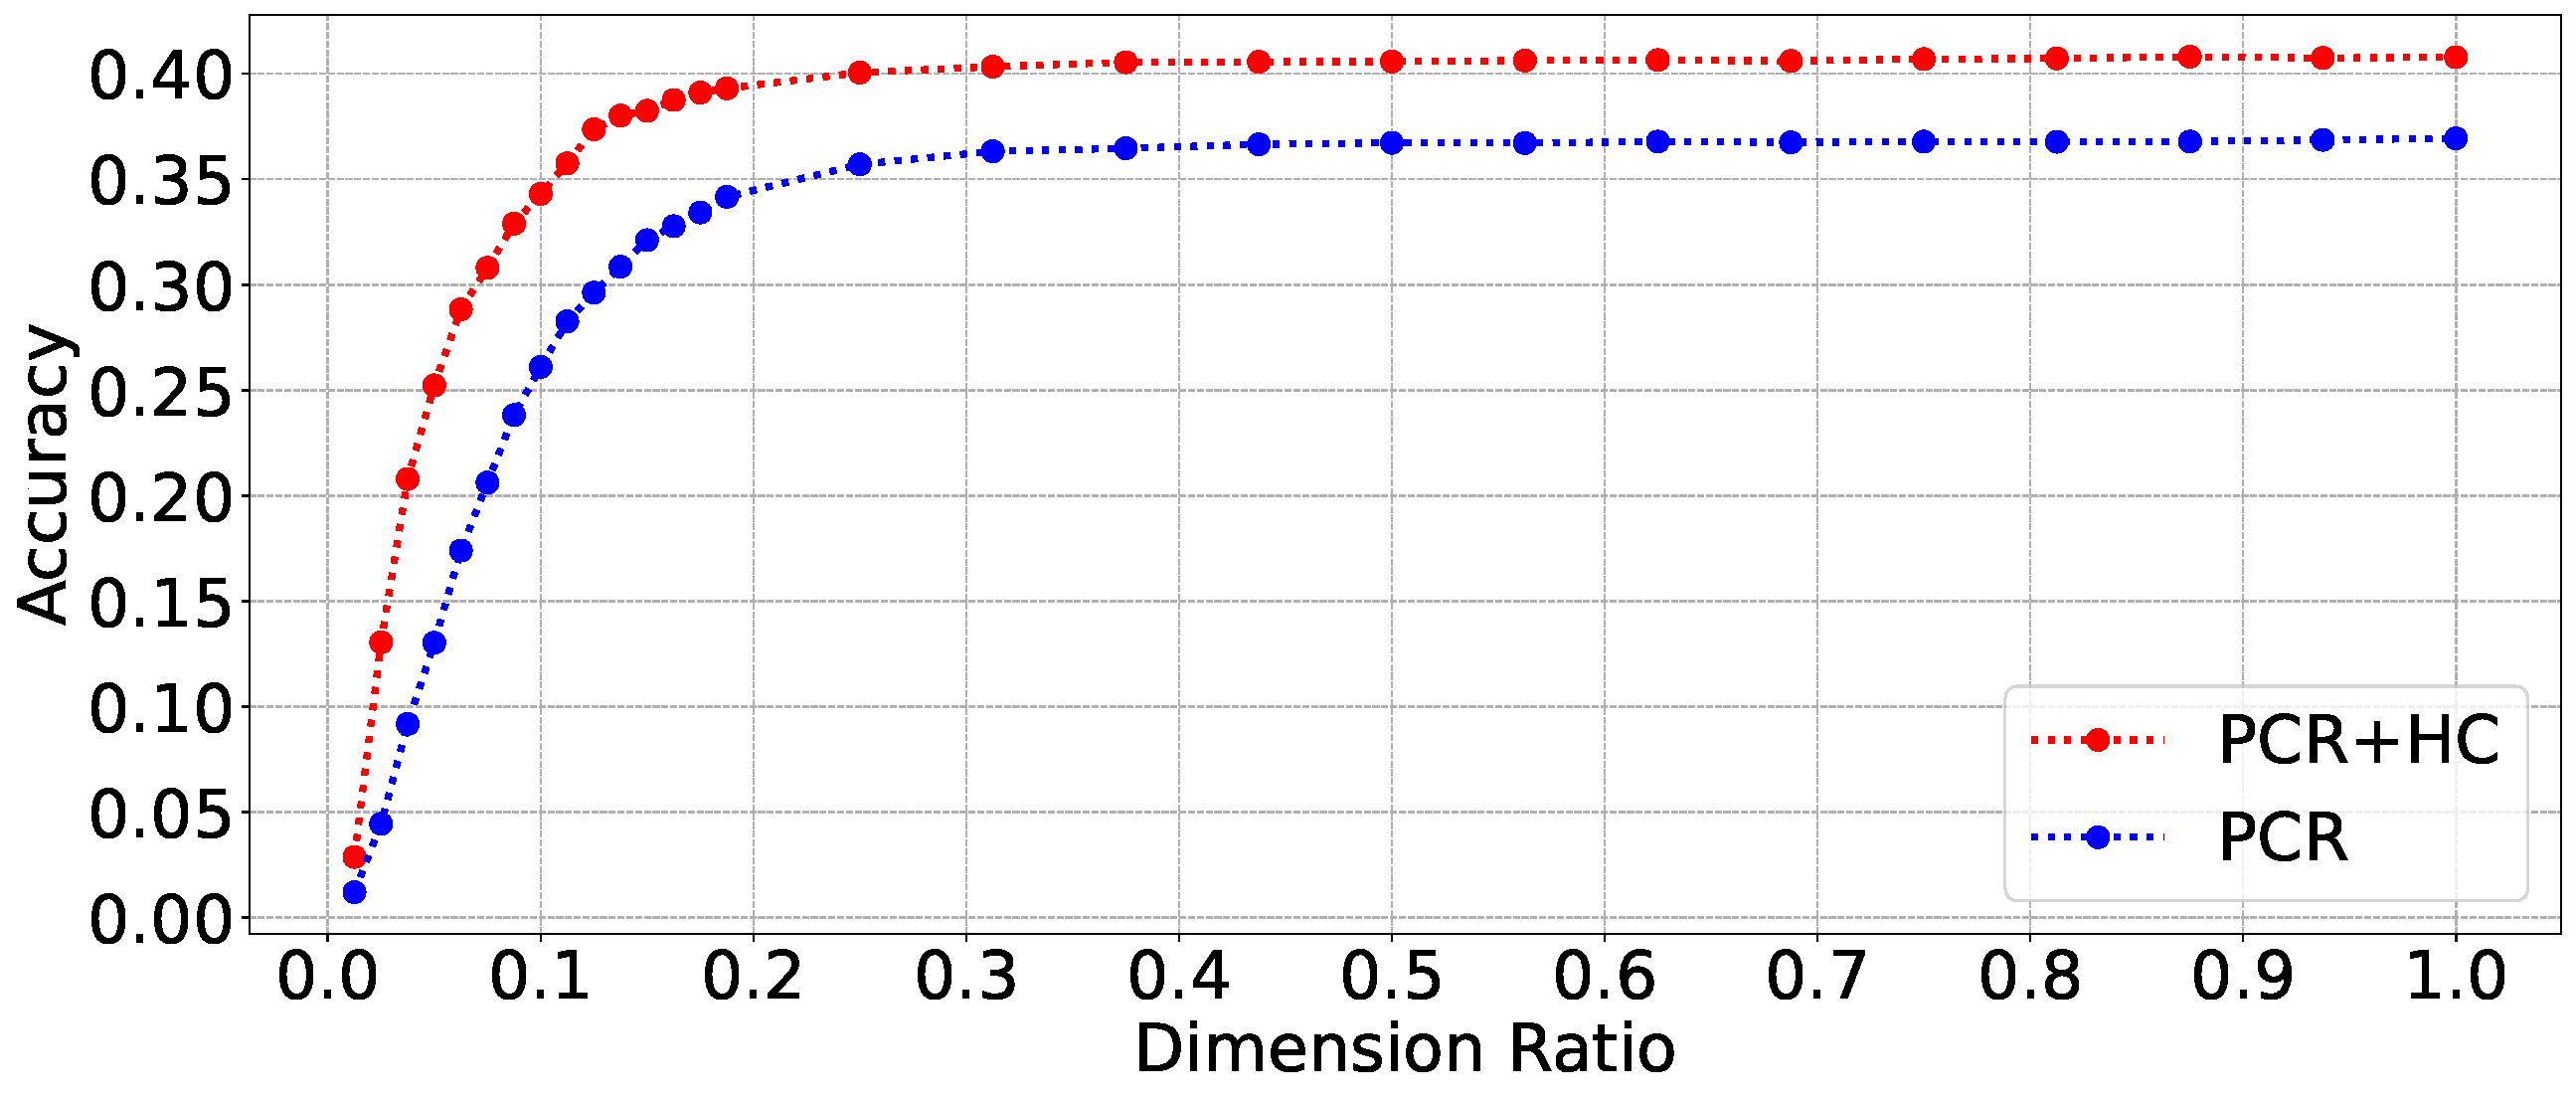
\includegraphics[scale=0.18]{sections/Figures/hpcr_cifar100_hc.pdf}
\vspace{-2ex}
\caption{Final Accuracy Rate on Split CIFAR100 (buffer size=5000) with different ratios of feature dimension.}
\label{fig:ablation_hc_pca}%
\vspace{-2ex}
\end{figure}

\begin{table}[t]
\renewcommand\tabcolsep{2.5pt}
\centering
\caption{Analysis results on CIFAR10 (buffer size=100) with and without temperature component.}
\vspace{-2ex}
\label{table:ablation_ht}
\begin{tabular}{l|lllll}
\hline
\makecell[l]{Different\\Setting} & \makecell[l]{Final\\Accuracy} & \makecell[l]{Cumulative\\gradient} & \makecell[l]{Loss} & \makecell[l]{Difference \\(all classes)} & \makecell[l]{Difference \\(new classes)} \\ \hline
w/o HT  & 42.83  & 88.27/-95.39    & 1.8439        & 0.0042     & 0.0056    \\
with HT & 47.66 & 64.28/-70.40    & 1.6710        & 0.0025     & 0.0040     \\ \hline
\end{tabular}
\vspace{-2ex}
\end{table}

\begin{figure}[t]
\centering
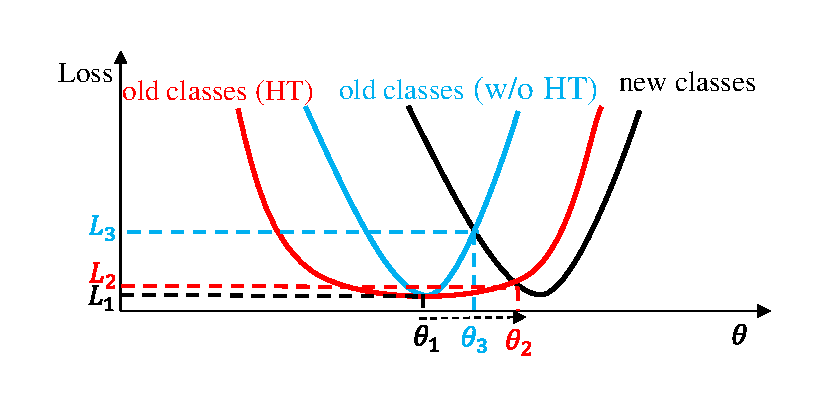
\includegraphics[scale=0.6]{sections/Figures/fig_ht.pdf}
\vspace{-2ex}
\caption{Illustration of a steep region not using HT and a flat region using HT.}
\label{fig:ablation_ht}%
\vspace{-2ex}
\end{figure}


\begin{table}[t]
\renewcommand\tabcolsep{2.5pt}
\centering
\caption{Accuracy Rate (higher is better) of HPCR on Split CIFAR100 with different $\tau_{min}$ and $\tau_{max}$ when the cycle length is 500. }
\vspace{-2ex}
\label{table:tau_step}
\begin{tabular}{l|lllll}
\hline
\diagbox{$\tau_{min}$}{$\tau_{max}$} & 0.12       & 0.14       & 0.16                & 0.18       & 0.2        \\ \hline
0.11  & 25.4, 34.9 & 25.0, 36.9 & 26.2, 36.6          & 26.3, 36.6 & 25.9, 36.7 \\
0.09  & 25.5, 35.8 & 26.0, 36.7 & 26.1, 36.9          & 26.5, 37.6 & 26.1, 37.8 \\
0.07  & 26.6, 36.8 & 26.3, 37.1 & 26.4, 37.6          & 26.2, 37.3 & 27.0, 38.1 \\
0.05  & 26.6, 37.1 & 26.7, 37.7 & \textbf{27.7, 38.5} & 26.9, 37.9 & 26.5, 37.6 \\ \hline
\end{tabular}
\vspace{-2ex}
\end{table}


\begin{table}[t]
\renewcommand\tabcolsep{2.5pt}
\centering
\caption{Accuracy Rate (higher is better) of HPCR on Split CIFAR100 with different cycle lengths $S$.}
\vspace{-2ex}
\label{table:tau_bound}
\begin{tabular}{l|llllll}
\hline
$S$ & 50   & 100  & 125  & 250  & 500  & 1000 \\ \hline
Final Accuracy   & 24.7 & 25.7 & 25.8 & 26.7 & \textbf{27.7} & 23.2 \\
Averaged Accuracy   & 34.6 & 36.5 & 36.8 & 37.8 & \textbf{38.5} & 32.4 \\ \hline
\end{tabular}
\vspace{-2ex}
\end{table}



\begin{table}[!h]
\renewcommand\tabcolsep{2.5pt}
\centering
\caption{Final Accuracy Rate (higher is better) of each task on Split CIFAR10 using distillation as DER or PCD.}
\vspace{-2ex}
\label{table:ablation_hd}
\begin{tabular}{l|llllll}
\hline
Task     & 1               & 2              & 3              & 4      & 5      & Average         \\ \hline
DER~\cite{buzzega2020dark} & 0.3480           & 0.2205         & 0.4320          & \textbf{0.5315} & \textbf{0.7500}   & 0.4564          \\
PCD (ours)      & \textbf{0.3695} & \textbf{0.2270} & \textbf{0.488} & 0.4960  & 0.7405 & \textbf{0.4642} \\ \hline
\end{tabular}
\vspace{-2ex}
\end{table}

\begin{figure}[t]
\centering
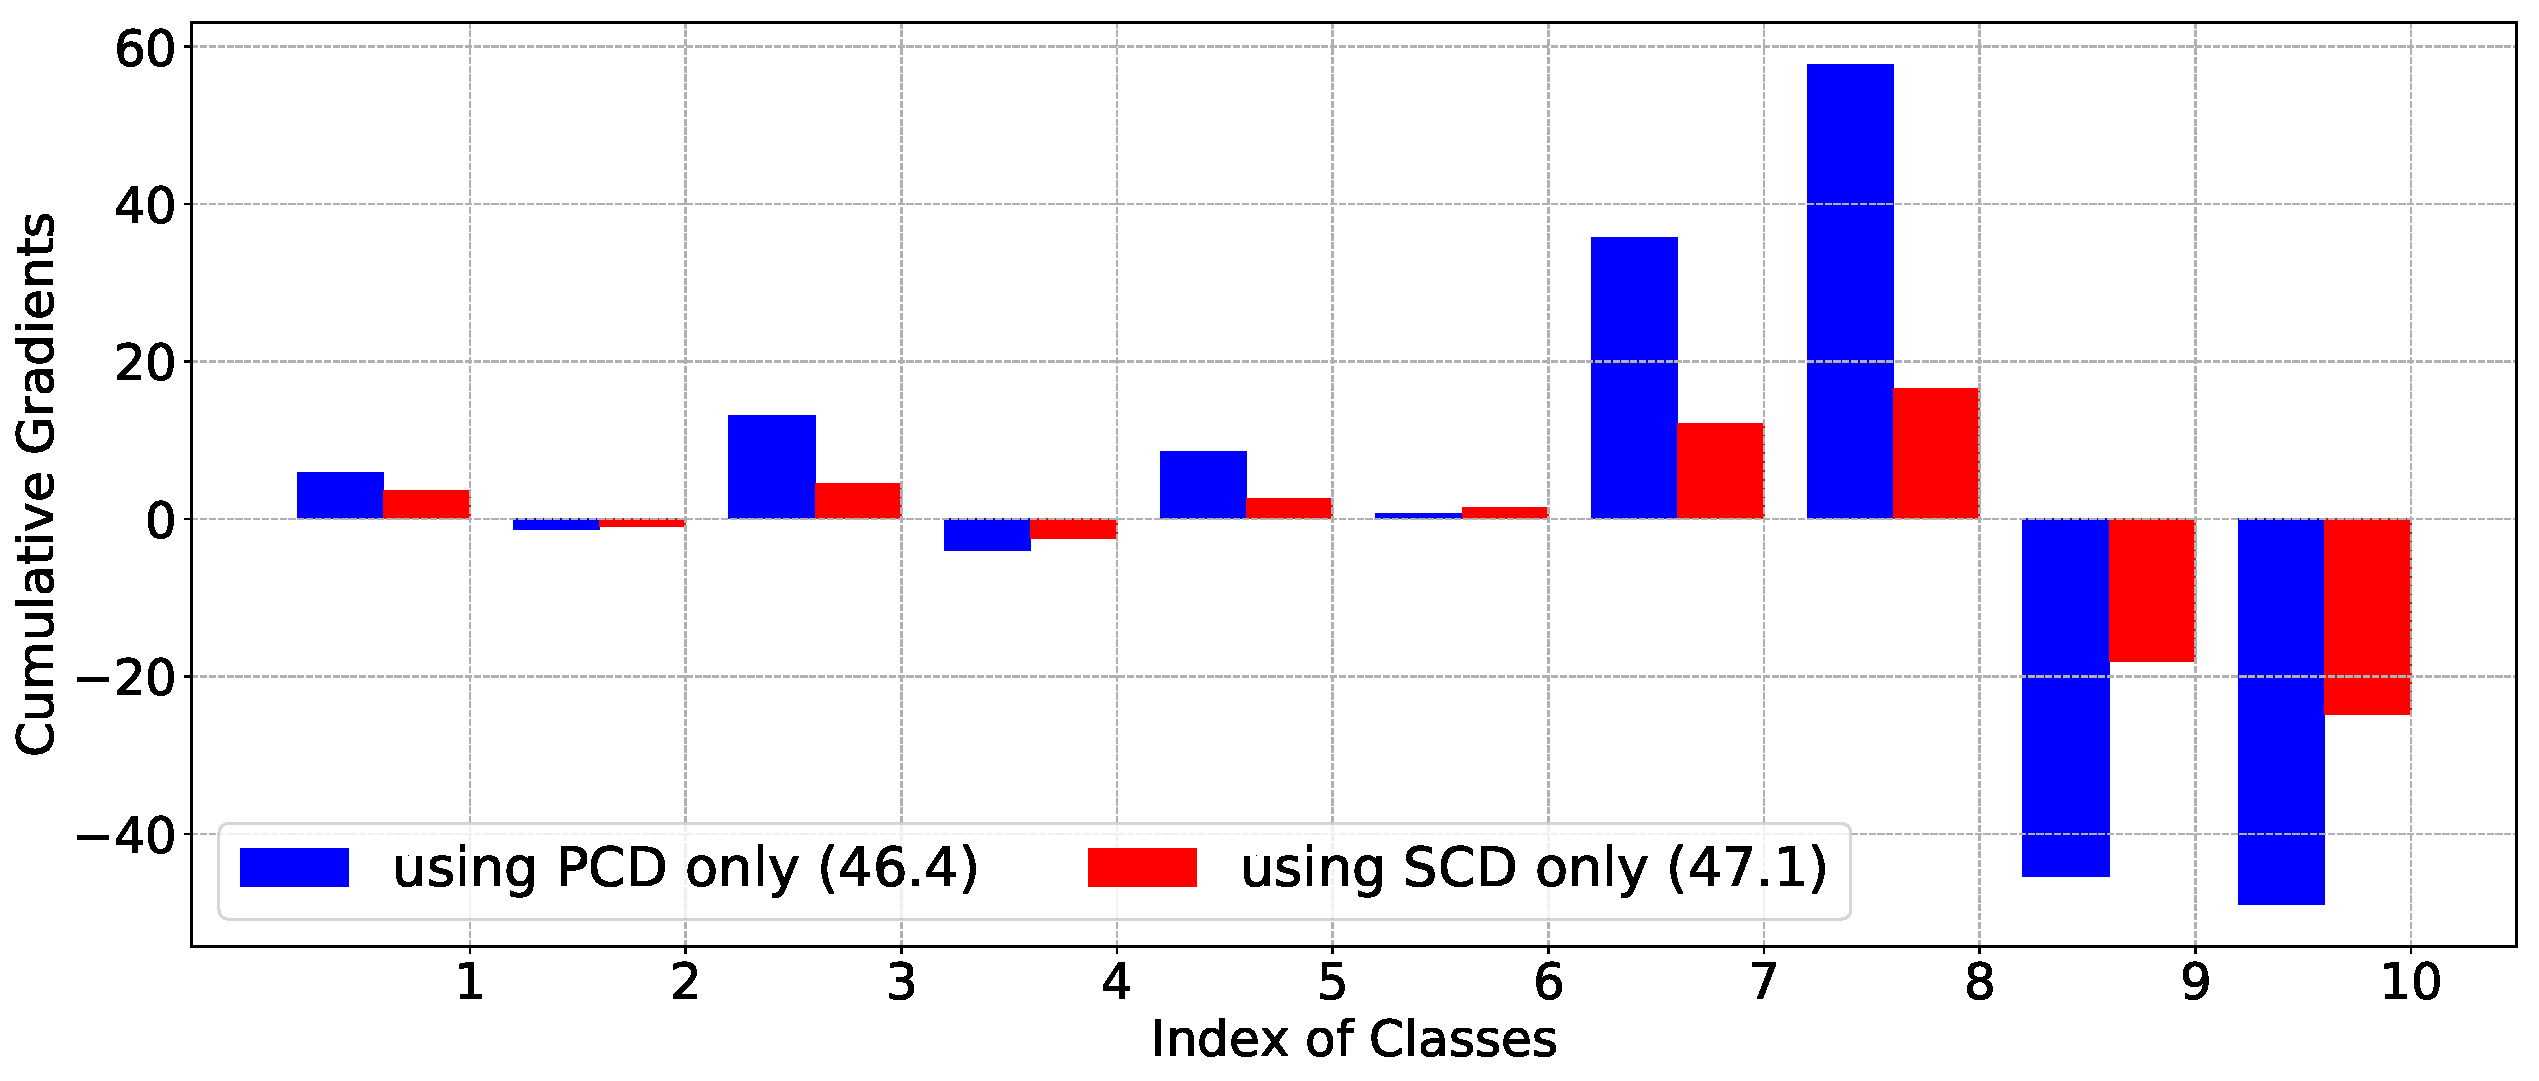
\includegraphics[scale=0.18]{sections/Figures/pcr_hd_gradient.pdf}
\vspace{-2ex}
\caption{Cumulative gradient for all proxies using different distillation loss functions when the model learns new classes (9/10) on Split CIFAR10.}
\label{fig:ablation_hd}%
\vspace{-2ex}
\end{figure}


\begin{figure}[t]
\centering
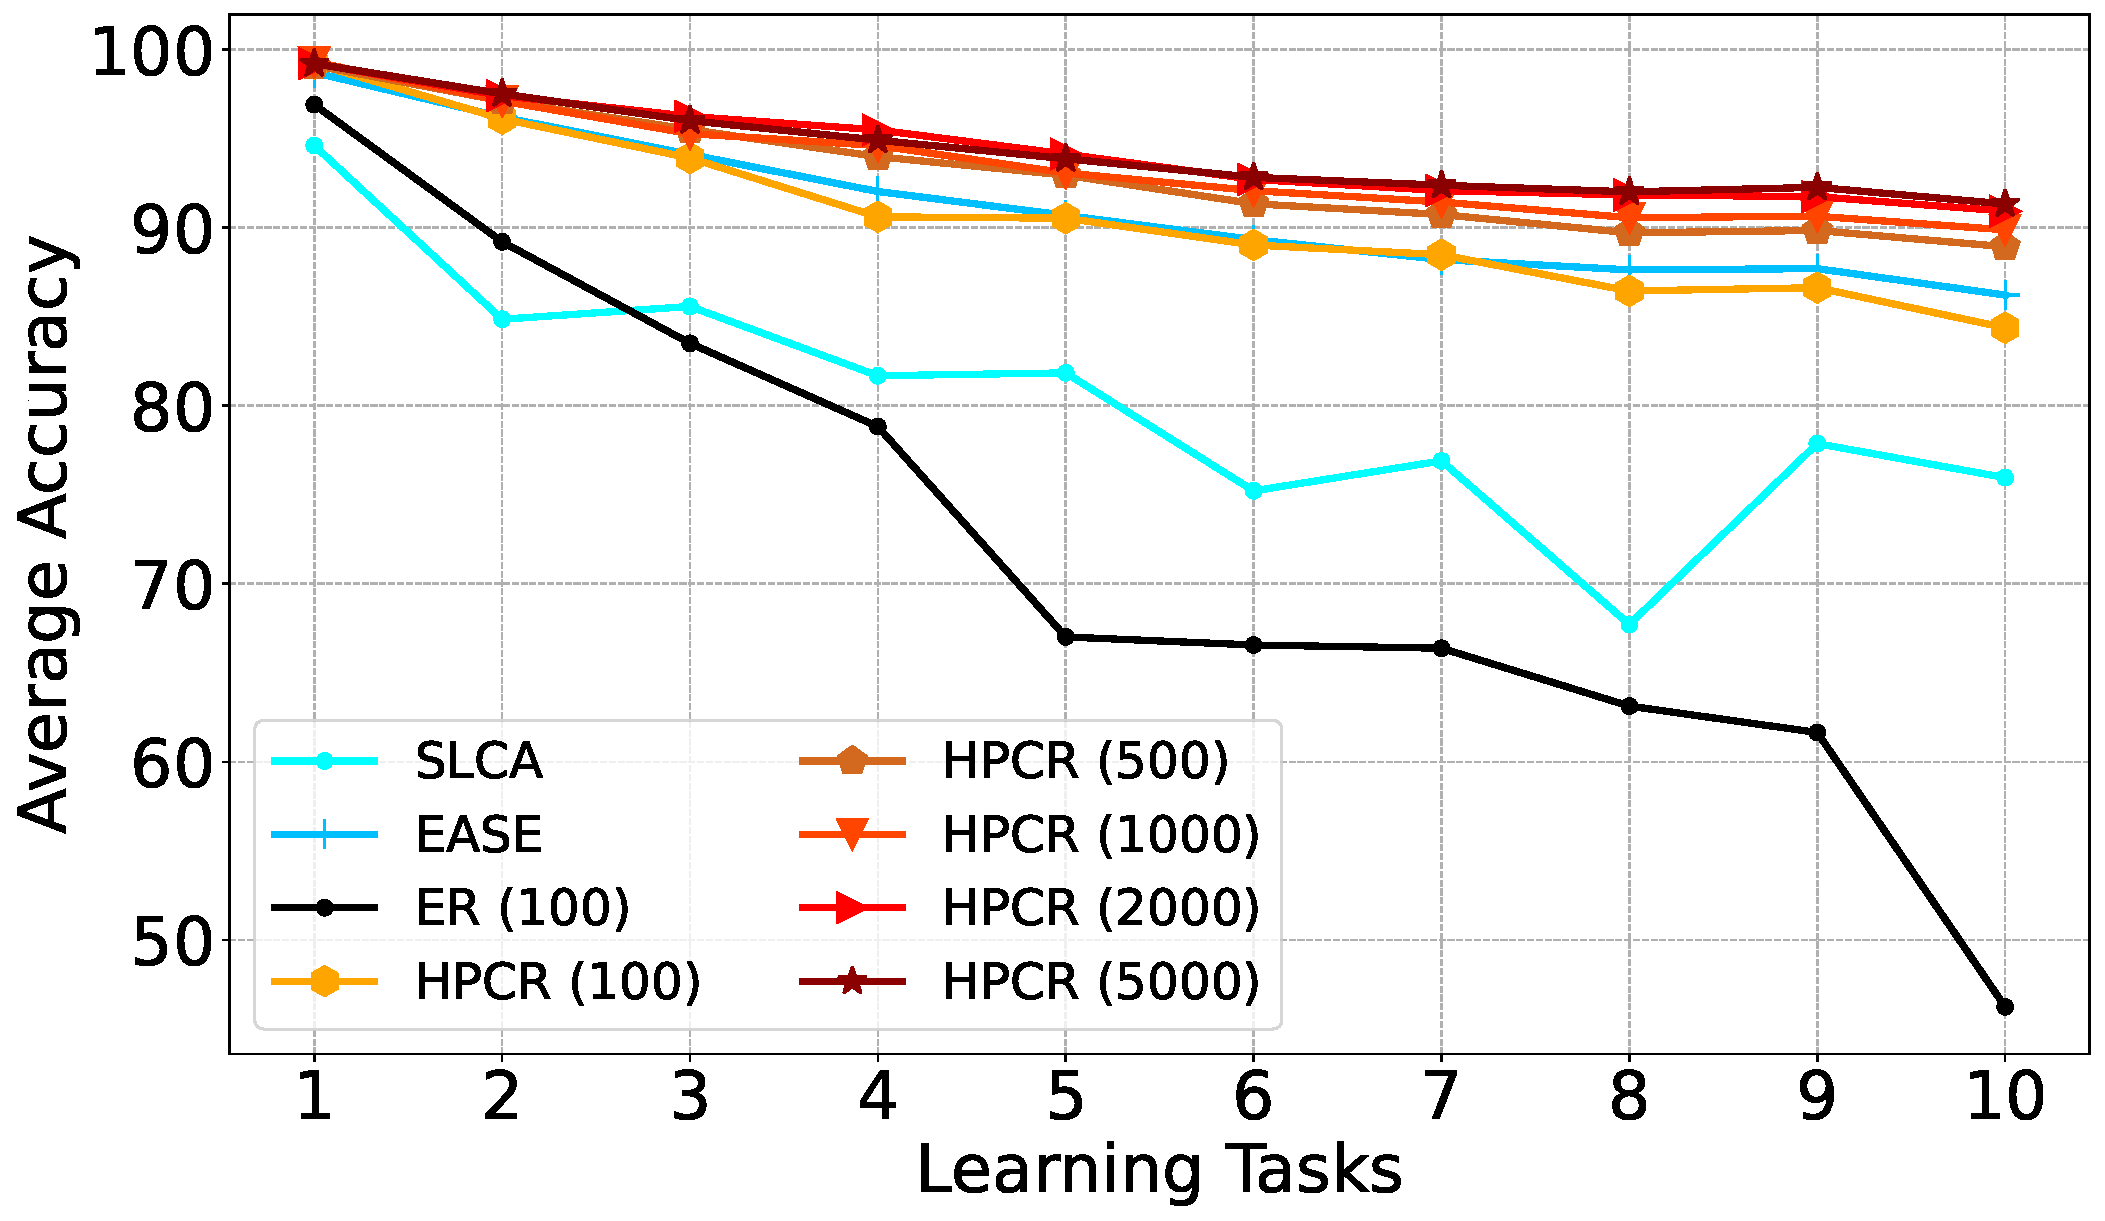
\includegraphics[scale=0.22]{sections/Figures/hpcr_cifar100_acc_pretrained.pdf}
\vspace{-2ex}
\caption{Average accuracy Rate on Split CIFAR100 with different methods.}
\label{fig:pretrained}%
\vspace{-2ex}
\end{figure}



\begin{figure}[!h]
\centering
\subfigure[ER (previous samples=10)]{
    \begin{minipage}[t]{0.46\linewidth}
        \centering
        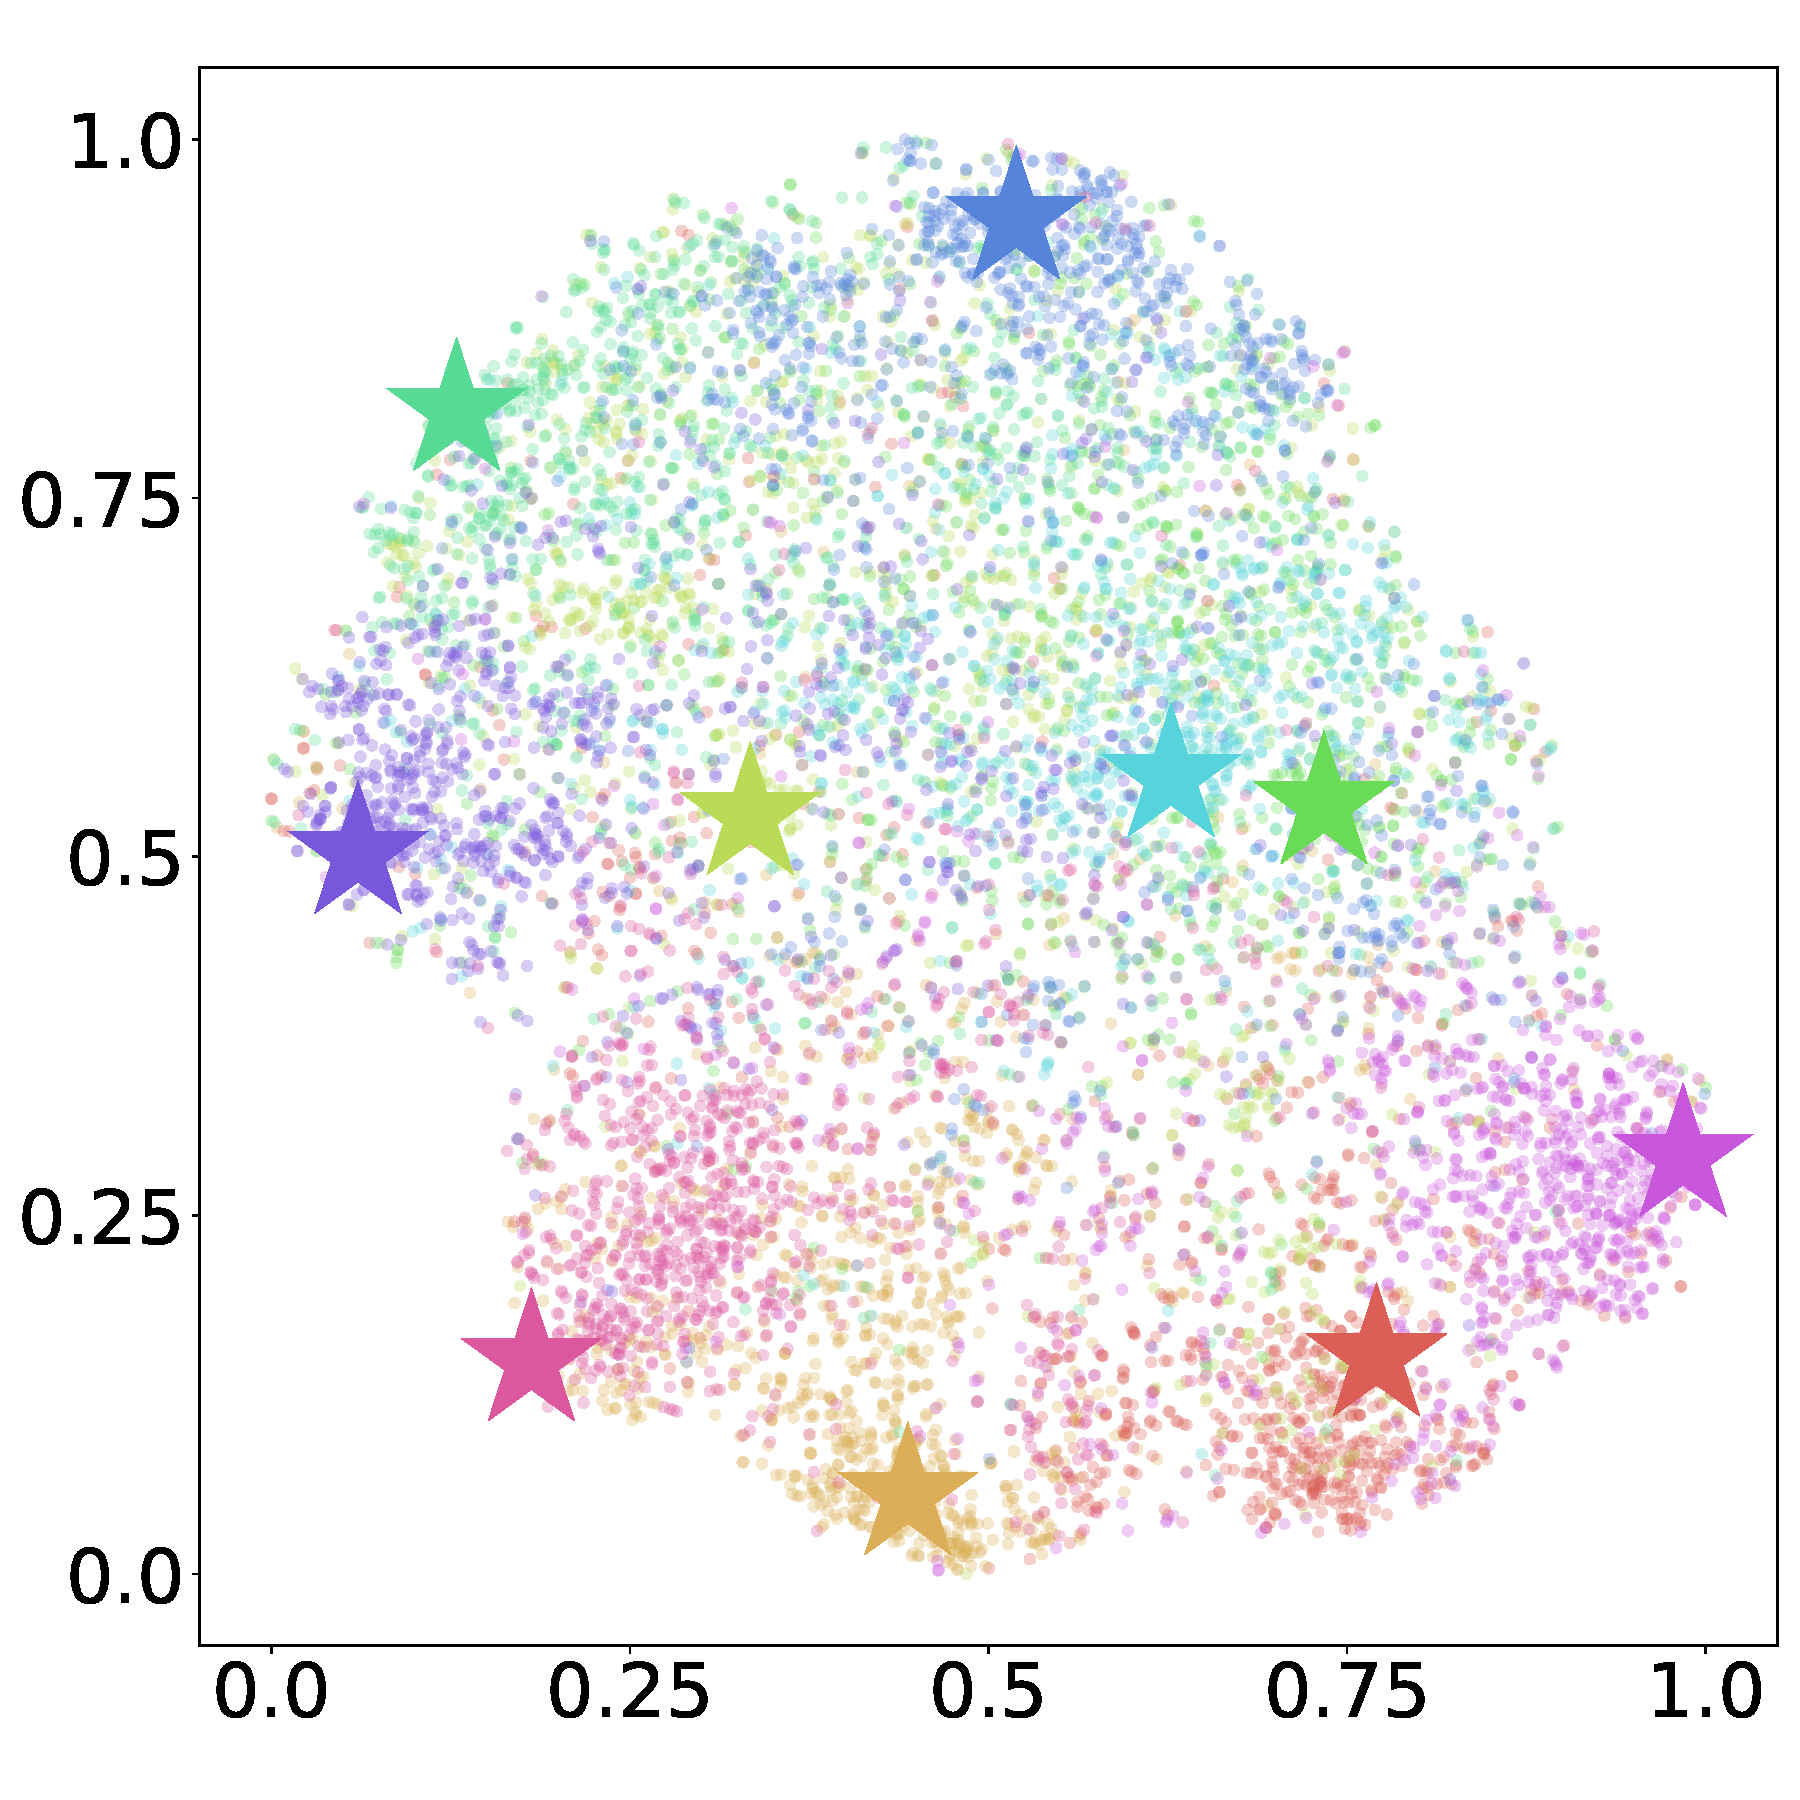
\includegraphics[scale=0.13]{sections/Figures/tsne_logits_er.pdf}
    \end{minipage}
}
\subfigure[ER (previous samples=100)]{
    \begin{minipage}[t]{0.46\linewidth}
        \centering
        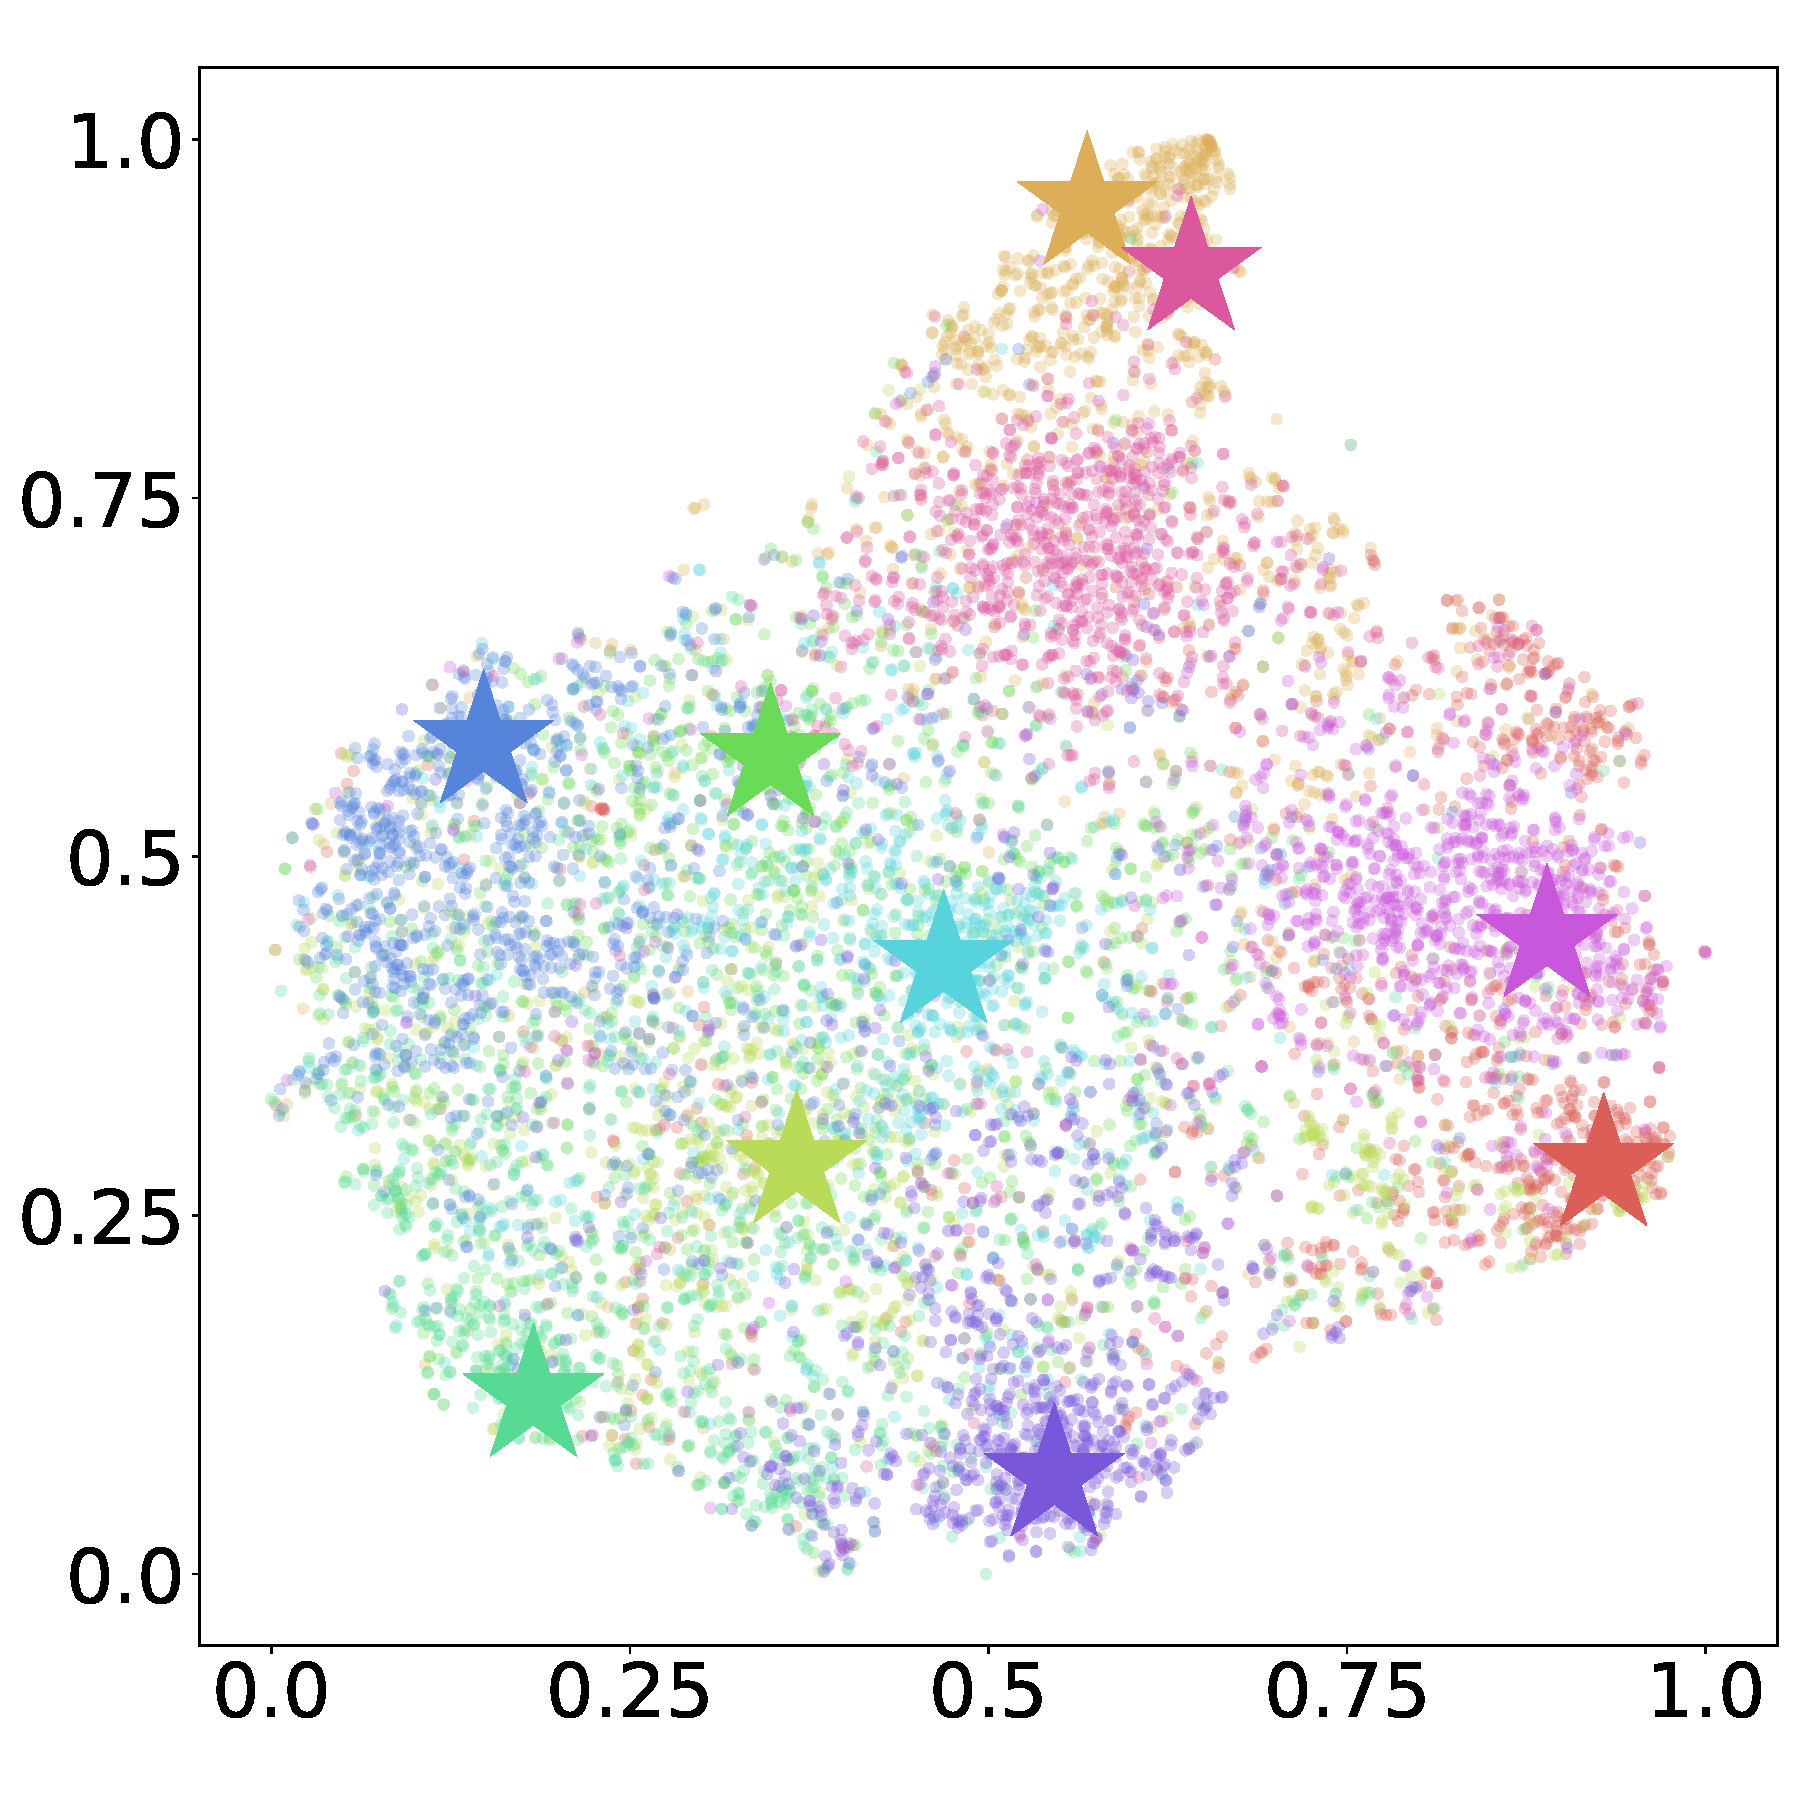
\includegraphics[scale=0.13]{sections/Figures/tsne_logits_er100.pdf}
    \end{minipage}
}
\centering
\subfigure[HPCR (previous samples=10)]{
    \begin{minipage}[t]{0.46\linewidth}
        \centering
        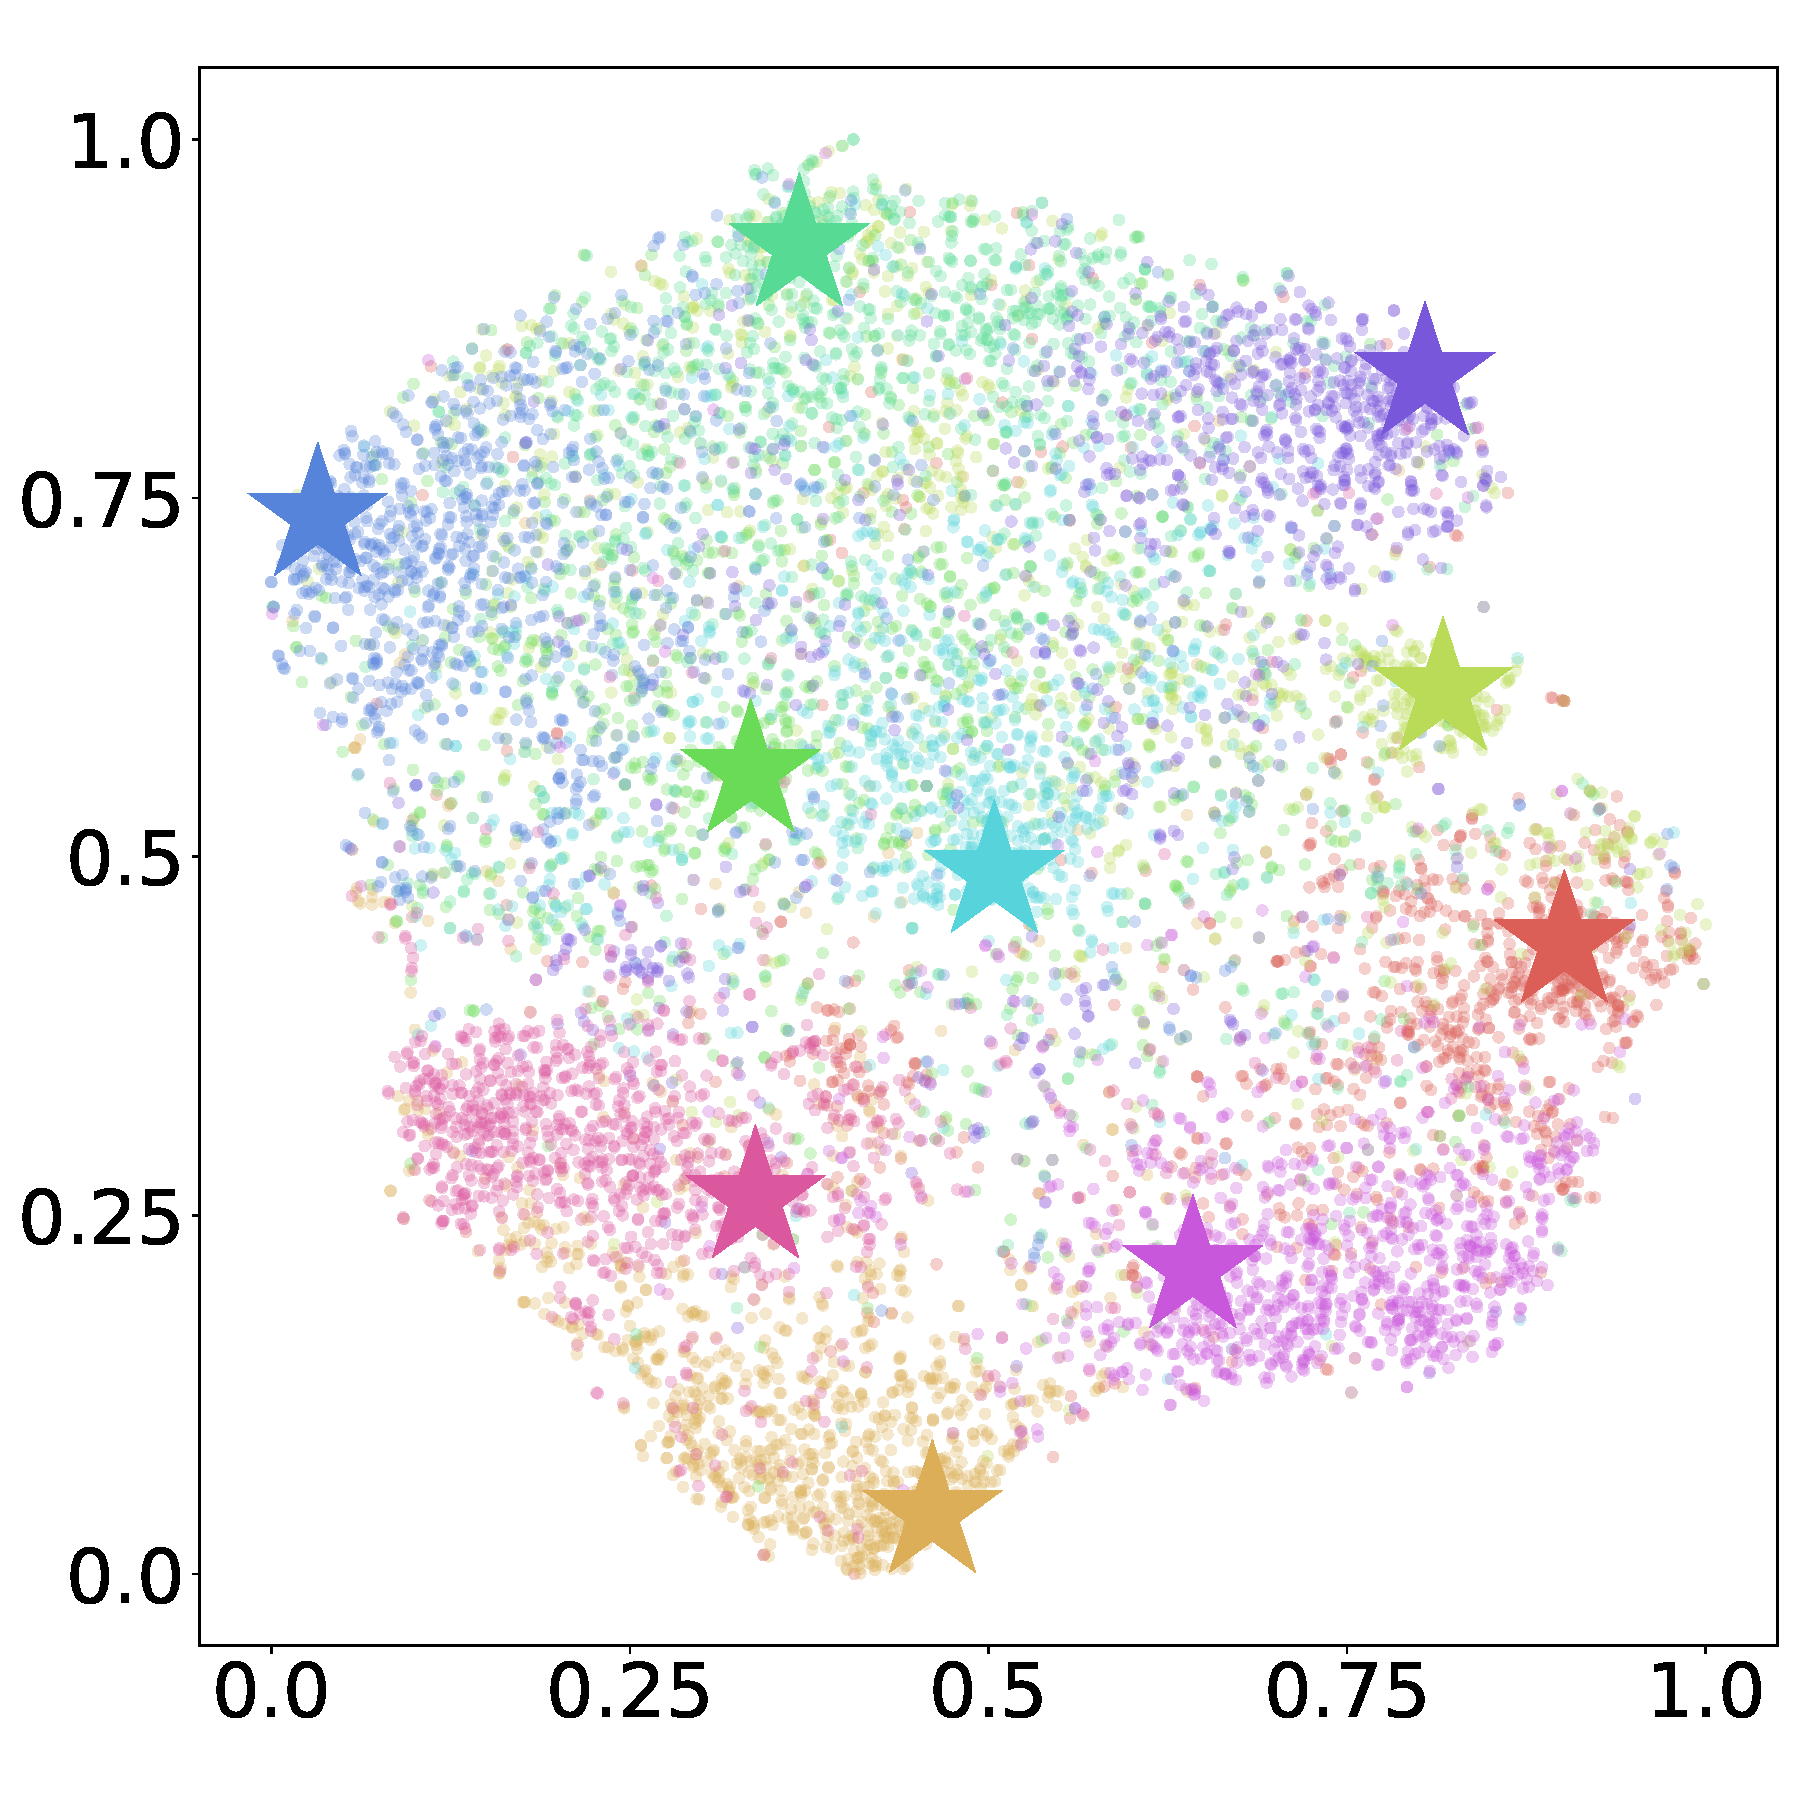
\includegraphics[scale=0.13]{sections/Figures/tsne_logits_hpcr.pdf}
    \end{minipage}
}
\subfigure[HPCR (previous samples=100)]{
    \begin{minipage}[t]{0.46\linewidth}
        \centering
        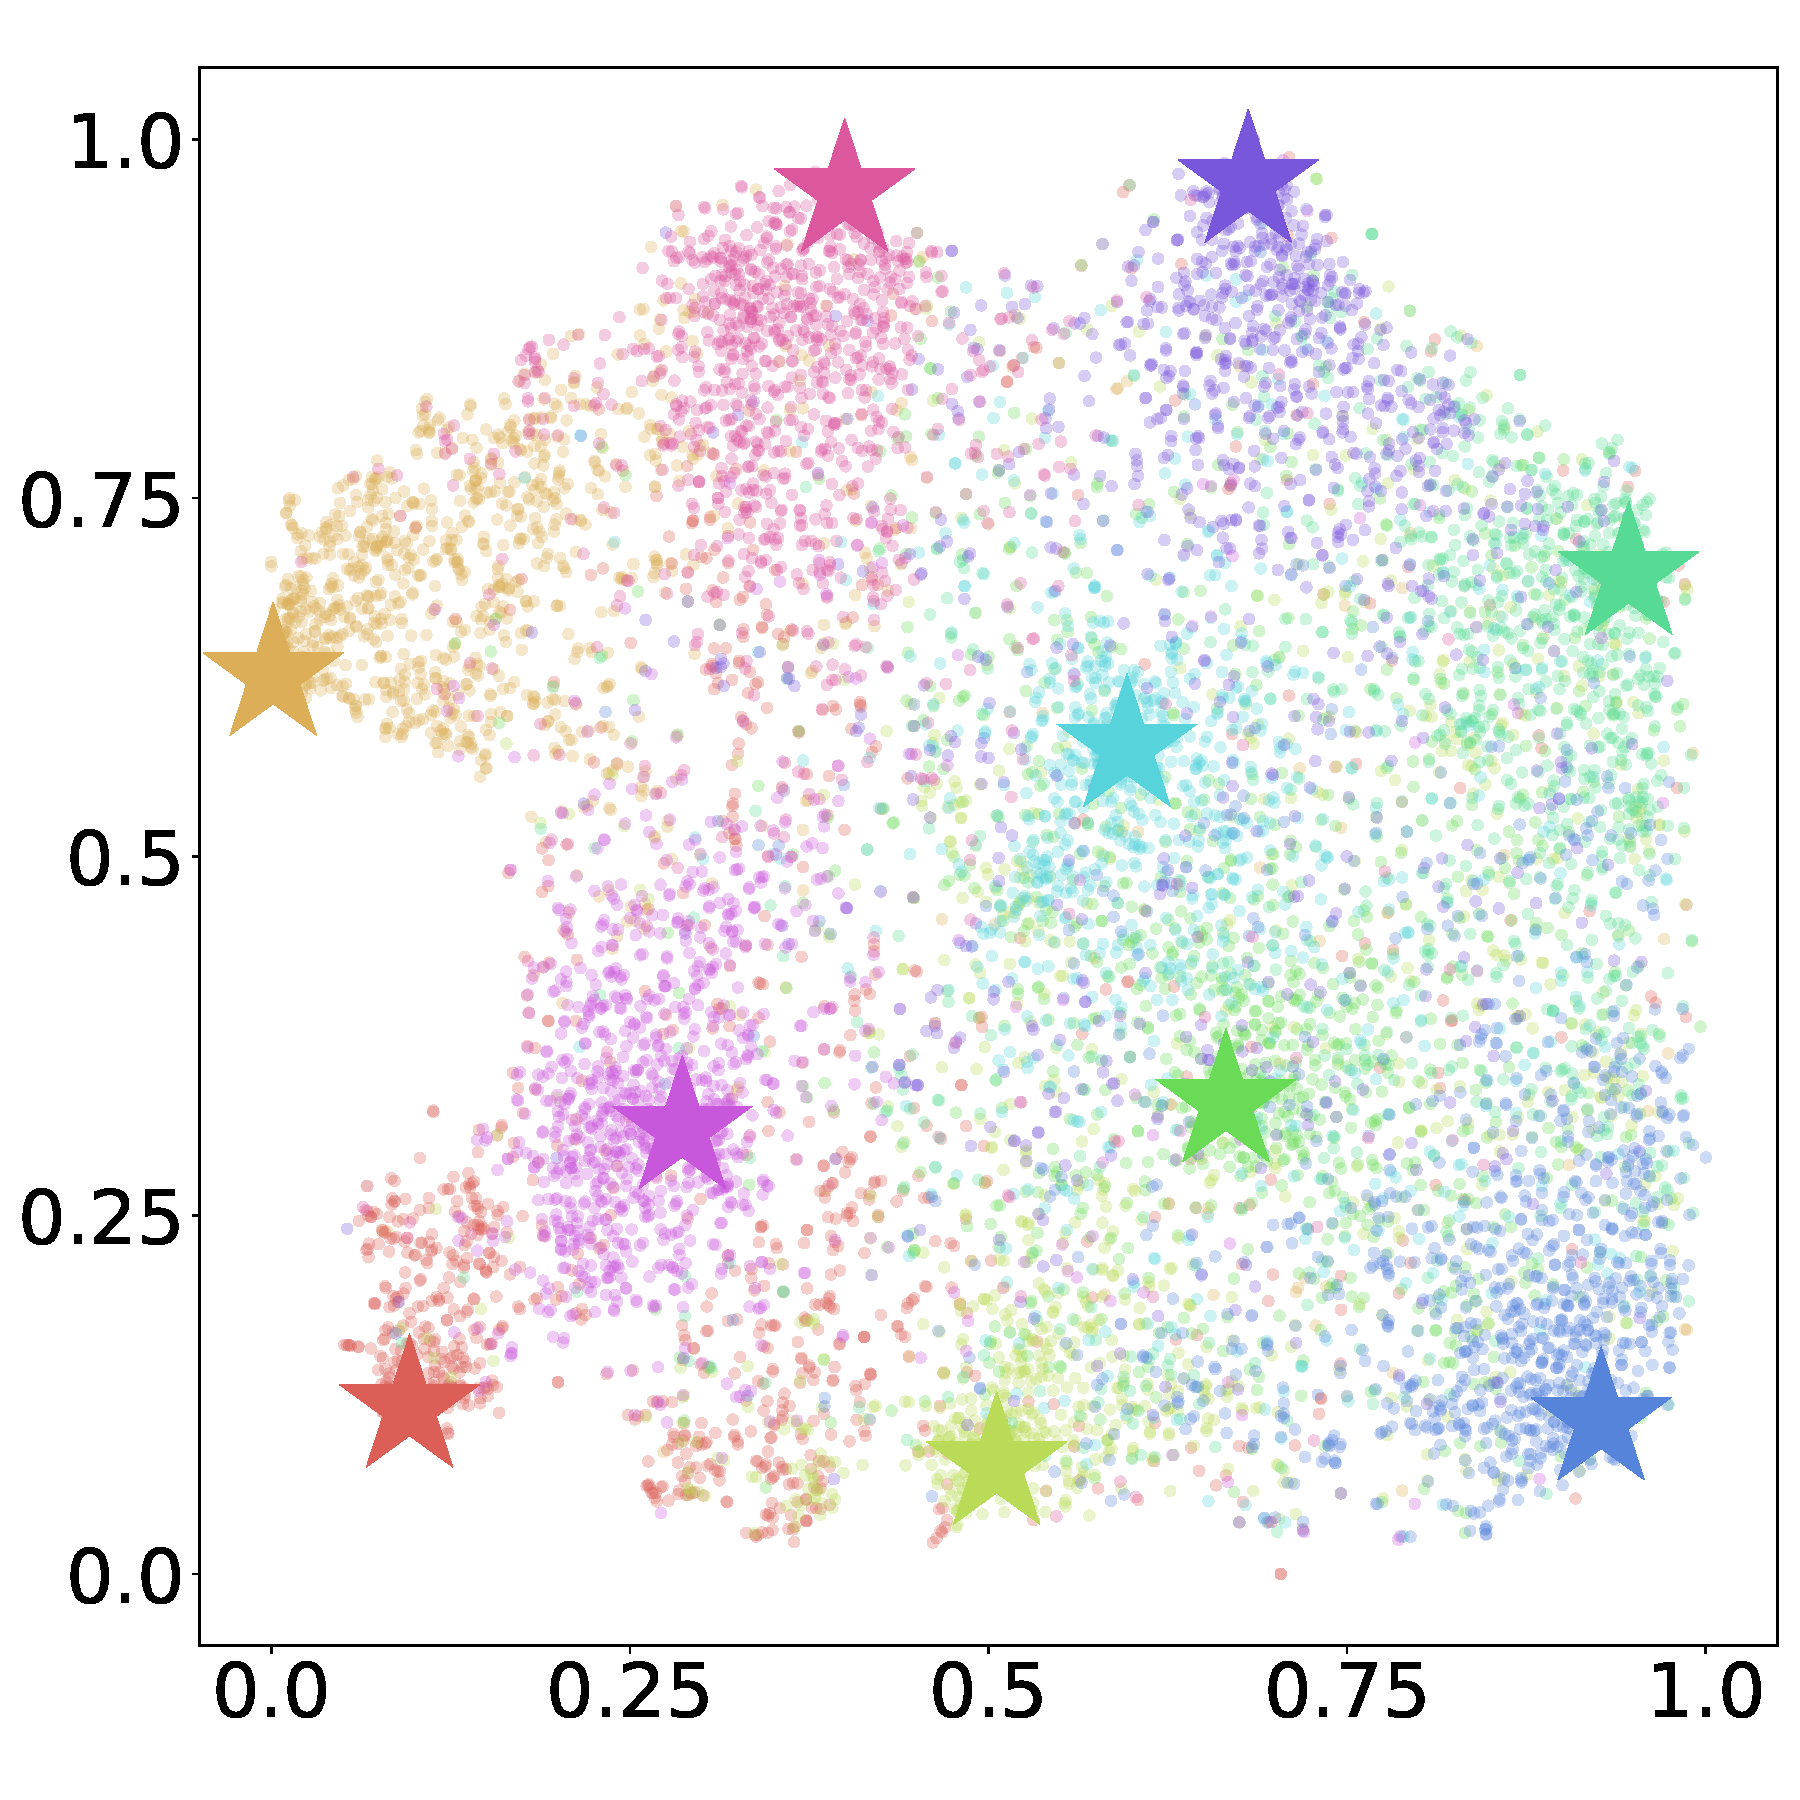
\includegraphics[scale=0.13]{sections/Figures/tsne_logits_hpcr100.pdf}
    \end{minipage}
}
\vspace{-1ex}
\caption{2D t-SNE visualization of feature embeddings for the testing samples at the end of the training on Split CIFAR10 (buffer size=500).} 
\label{fig:tsne}
\vspace{-3ex}
\end{figure}

\begin{table}[t]
\renewcommand\tabcolsep{2pt}
\centering
\caption{The computation and memory budget of different methods.}
\vspace{-2ex}
\label{table:other}
\begin{tabular}{l|ccccccc}
\hline
Method       & ER      & ER-ACE & OCM & OnPro & UER & PCR & HPCR\\ \hline
Computation ($C_\mathcal{D}$)       & 1      & 1 & 16 & 16 & 1 & 1 & 1\\
Memory (Model)       & 1      & 1 & 2 & 1 & 1 & 1 & 1\\
Memory (Data)       & 1      & 1 & 1 & 1 & 1 & 1 & Table~\ref{table:memory}\\
\hline
\end{tabular}
\vspace{-2ex}
\end{table}

\begin{table}[t]
\renewcommand\tabcolsep{2pt}
\centering
\caption{The memory (data) on different datasets for HPCR.}
\vspace{-2ex}
\label{table:memory}
\begin{tabular}{l|cccc}
\hline
Dataset       & CIFAR10      &CIFAR100  & MiniImageNet & TinyImageNet\\ \hline
Sample Size       & 32×32×3      & 32×32×3 & 84×84×3 & 64×64×3\\
Feature Size        & 160      & 160 & 640 & 640\\
Logits Size       & 10      & 100 & 100 & 200\\
Memory (Data)       & 1.06      & 1.08 & 1.03 & 1.07\\
Buffer Size     & 100      & 1000 & 1000 & 2000\\
Accuracy (Control)       & 47.7\scriptsize±1.5      & 27.4\scriptsize±0.5 & 26.5\scriptsize±0.6 & 15.2\scriptsize±0.4\\
Accuracy (HPCR)       & 48.3\scriptsize±1.5      & 29.1\scriptsize±0.7 & 27.1\scriptsize±0.6 & 16.4\scriptsize±0.3\\
\hline
\end{tabular}
\vspace{-4ex}
\end{table}

\subsection{Ablation Study}
In this section, we decompose HPCR into several components and demonstrate their functions. We conduct experiments with different settings and record their final accuracy rate in Table~\ref{ablation}. In addition to ER, we also include the two combination methods denoted as Equation (\ref{eq:coupleloss1}) and Equation (\ref{eq:coupleloss2}). The experimental results show that they are not significant since they do not solve the problem of forgetting.   

% \subsubsection{The Components of PCR}

% The \textbf{selection component} (PS) is the basic component of PCR, which selects the anchor-to-proxy pairs in the contrastive-based replay manner. Actually, there are some samples from the same classes in a training batch. As a result, there are some duplicate anchor-to-proxy pairs in PCR. To effectively verify the role of the selected proxies, we remove the duplicate pairs. As shown in Table~\ref{ablation}, the performance of ER is significantly improved with the help of this component.

% The other component is a \textbf{duplication component} (PD) to keep the duplicate pairs in PCR. Although it contains the same knowledge as the anchor-to-proxy pairs in the selection component, it still produces significant performance. Since it can provide anchor samples with more negative pairs, which are vital to contrastive-based loss. As described by the gradient analysis of PCR in Section~\ref{sec:PCR}, the number of duplicate pairs will be used as the weight of pairs for the probability distribution calculation of the sample. This weight not only reduces the negative gradient of the current sample towards other classes, but also increases the positive gradient of a previous sample towards its class.  As stated in Table~\ref{ablation}, PCR outperforms ``ER+PS'' with the duplication component PD.

% The \textbf{classifier component} (PC), which replaces the softmax classifier by the NCM classifier for PCR, is a less important part. Before testing, the NCM classifier requires recalculating the feature vectors of previous samples in the buffer to obtain the final classifier. Compared to the original classifier, it requires additional time and operation, which is unfavorable for OCL. As demonstrated in Table~\ref{ablation}, the combination of PCR and NCM classifier is not necessarily the best. The NCM classifier is more suitable for situations with smaller samples
% (e.g. Split-CIFAR100) and a larger buffer. Since small-sized samples are easy to obtain reliable features, and large-sized buffer trends to obtain accurate classification centers.

% In conclusion, the selection component and the duplication component are the keys of PCR. As displayed in Figure~\ref{fig:gradient}, PCR produces uniform gradients for all proxies to address the ``bias'' issue by the smart selection of anchor-to-proxy pairs. Furthermore, since the way of selection depends on the classes in the training batch, PCR is influenced by the batch size. Figure~\ref{fig:batch} reports the performance of several methods with different batch sizes. With the increase in batch size, PCR consistently maintains its advantages.

% \subsubsection{The Components of HPCR}

\textbf{Contrastive component} (HC) conditionally incorporates anchor-to-sample pairs to PCR. Although it provides more knowledge about the relationships of samples, its performance is limited by a small batch size of training samples, as the ``PCR+HC'' indicated in Table~\ref{ablation}. Meanwhile, we conduct experiments on Split CIFAR100 using PCR with and without HC. The results revealed in Figure~\ref{fig:ablation_hc} show that the anchor-to-sample pairs can reduce the performance of PCR when the batch size of the training samples is small ($<60$), and vice versa. Hence, the usage of anchor-to-sample pairs should be controlled by a stage function denoted as Equation (\ref{eq:step_function}). To further explore HC, we conduct principal component analysis (PCA)~\cite{wold1987principal} on the features $\bm{z}$ extracted by the model. As demonstrated in Figure~\ref{fig:ablation_hc_pca}, we report the final accuracy rate on Split CIFAR100 with different ratios of feature dimension when the batch size of previous samples is 100. In cases where the dimension ratio is low, ``PCR+HC'' performs much better than PCR, and this advantage is maintained as the ratio increases. It means that the feature extraction capability of the model has been improved with the help of HC, allowing for the extraction of more critical features.

\textbf{Temperature component} (HT) is to improve the model's generalization ability. As stated in Table~\ref{ablation}, with the help of HT, the performance of PCR is greatly improved. Compared with ``PCR'' and ``PCR w/o HD'' in Figure~\ref{learningstage5000}, we find that the main improvement brought by HT lies in learning novel knowledge by the model. To explore the role of HT on gradient propagation and model convergence, we analyze the training process of PCR on the CIFAR10 with and without HT, and some important indicators are recorded in Table~\ref{table:ablation_ht}. The results show the final accuracy can be improved by HT since the model can produce less gradient for old classes ($64.28<88.27$) and new classes ($70.40<95.39$) during the gradient propagation process. In the meantime, we find that HT can make the model converge to a region with a lower loss function value ($1.6710<1.8439$) and a flatter landscape during the optimization process. To validate it, we add uniformly distributed noise to the parameters of the final model, causing the position of the model to change in the parameter space. At the same time, we record the differences in training loss before and after the model changes. After repeating the above operations 1000 times, we calculate the average of these 1000 results. The results indicate that the model has relatively small differences using HT for all classes ($0.0025<0.0042$) and new classes ($0.0040<0.0056$). Therefore, the optimal solution of the model using HT is in a relatively flat region. As displayed in Figure~\ref{fig:ablation_ht}, in such a flat region, the model, where the initial solution is $\theta_1$, can obtain a better solution $\theta_2$ than $\theta_3$ for both old and new classes. Moreover, the selection of hyperparameters related to Equation~(\ref{eq:tau_t}) is shown in Tables~\ref{table:tau_step} and \ref{table:tau_bound}. And we set $\tau_{max}=0.16$, $\tau_{min}=0.05$, and $S=500$ based on the results. 






\textbf{Distillation component} (HD) is to improve the anti-forgetting ability of the model. Compared with ``HPCR'' and ``HPCR w/o HD'' in Figure~\ref{learningstage5000}, we can find that HPCR performs significantly better on historical knowledge with the help of HD. Shown as Table~\ref{ablation}, the distillation component, which contains SCD and PCD, further improves the performance of PCR. To improve the overall performance of the model, both SCD and PCD are essential. For one thing, SCD can better balance the distribution of historical knowledge while improving the model's ability to anti-forgetting. Actually, there is an imbalance between old classes in OCL. As shown in Table~\ref{table:ablation_hd}, although tasks 1-4 are all old tasks, the performance of the model on these tasks is different. Compared with the distillation method in DER, PCD can better balance the performance of the model on old tasks (Tasks 1-4). For another thing, SCD, which directly propagates gradient for feature extractor, can produce less gradient for all proxies than PCD. As shown in Figure~\ref{fig:ablation_hd}, if HPCR only uses SCD, the gradient is relatively small, and the final performance is better.

In summary, based on these three components, HPCR has a comprehensive improvement compared to PCR. At the same time, all of the components are tailored to break the limitations of PCR and have their own originality.


 

\subsection{Further study}

\subsubsection{Pre-trained Backbone} With the development of pre-trained models, continual learning tends to take a pre-trained model as the initial model. Hence, we further conduct experiments with a pre-trained model on Split CIFAR100. For fairness, we consider the ViT-B/16-IN21K in~\cite{zhou2024expandable} as the pre-trained model, where each frozen transformer block contains a trainable residual term. Meanwhile, the training batch size is set as 10 and the epoch is set as 1 for all methods. As stated in Figure~\ref{fig:pretrained}, SLCA~\cite{zhang2023slca} and EASE~\cite{zhou2024expandable} are non-replay methods while ER replays with a 100-size buffer. Compared with ER (100) and HPCR (100), we can find that HPCR can also play a role when using a pre-trained backbone. Moreover, the performance of HPCR will gradually surpass SLCA and EASE based on pre-trained models as the buffer size increases (from 100 to 5000), further confirming its superiority for OCL.

\subsubsection{Visualization} Visualization can
help reflect the role of these components more intuitively. We train the model by ER and HPCR on Split CIFAR10 with 500 sizes of memory buffer, respectively. At the end of the training, we report their 2D t-SNE~\cite{van2008visualizing} visualization of feature embeddings for all testing samples, as shown in Figure~\ref{fig:tsne}. The stars are proxies while others are samples for all classes. The results demonstrate that HPCR not only achieves great performance, but also can indeed improve the distinguishability of samples in the embedding space.


\subsubsection{Computation and Memory Cost} For OCL, the overhead of memory and computing resources is crucial, since it will affect the practicality of a method. Therefore, we analyze the memory and computational cost of different methods, as reported in Table~\ref{table:other}. 1) Similar to~\cite{ghunaim2023real}, we use $C_\mathcal{D}$ to compare the computation of different methods. The $C_\mathcal{D}$ is denoted as a relative complexity between the stream and an underlying continual learning method. For example, when current samples come, ER can immediately learn them and then predict unknown samples, resulting in a relative complexity of 1. Since UER, ER-ACE, PCR, and HPCR only modify the loss objective of ER, their computational complexities are equivalent to 1. However, OCM and OnPro require an additional 16 augmentation to the original data, making it require 16  times the FLOPs needed by ER. Thus, its computational complexity is 16, which limits the ability of real-time prediction. 2) We set the memory budget of the model for ER as 1. Due to the OCM method requiring an additional model to be saved for knowledge distillation, its relative budget is 2 and others are 1. 3) We evaluate the memory usage of different methods by considering the data size of all samples stored in the buffer. As seen in Table~\ref{table:memory}, since HPCR has additional storage requirements for features and logits embedding, it necessitates relatively more memory space ($>1$). However, the additional memory does not occupy a high proportion ($<0.1$). If the additional memory is used to store old samples, the performance of the model is shown in the row of ``Accuracy (Control)''. The results demonstrate that storing features and logits as HPCR yields significant benefits, justifying its worth. In summary, HPCR emerges as a straightforward yet efficacious approach for real-time prediction in OCL scenarios.



